\documentclass[10pt,a4paper]{article}
\usepackage{setspace,epsfig,harvard,xspace}
\usepackage{amsmath}
\citationstyle{dcu}
\citationmode{abbr}
\pretolerance400
\tolerance800
\emergencystretch2em
\doublehyphendemerits5000
\hfuzz0pt
\leftskip0pt minus 1pt
\rightskip0pt minus 1pt
\parskip=6pt
\newcommand{\IE}{\textit{i.e.},\xspace}
\newcommand{\EG}{\textit{e.g.},\xspace}
\newcommand{\GT}{\ensuremath{\mathcal{G}}\xspace}
\newcommand{\Th}[1]{#1\textit{th}\xspace}
\newcommand{\MCMC}{Markov chain Monte Carlo}
\newcommand{\Prep}{\texttt{prep}\xspace}
\newcommand{\Loki}{\texttt{loki}\xspace}
\newcommand{\Lokiext}{\texttt{loki\_ext}\xspace}

\addtolength{\oddsidemargin}{-.5in}
\addtolength{\textwidth}{1in}
\addtolength{\topmargin}{-.5in}
\addtolength{\textheight}{1in}
\renewcommand{\refname}{References}
\renewcommand{\figurename}{Figure}
\parindent=0pt

\begin{document}
\thispagestyle{empty}
\begin{center}
\begin{Large}
\textbf{Loki 2.4.6}\\[.15in]
A package for multipoint linkage analysis on large pedigrees using
Reversible jump Markov chain Monte Carlo\\[.25in]
\end{Large}
\begin{large}
April 2003\\[4.5in]
\end{large}
\end{center}
Simon C Heath\\ 
Centre National de G\'enotypage\\
2 rue Gaston Cr\'emieux\\
CP 5721, 91057 Evry Cedex
France\\[.1in]
email: \verb+heath@cng.fr+\\
\newpage
\section{Overview}
The programs described here are an implementation of the methods described in
\citeasnoun{heath_97a} for Markov chain Monte Carlo (MCMC) segregation and linkage
analysis of quantitative traits using oligogenic models.  The programs are
intended for performing multipoint linkage analyses on large, possibly
complex, pedigrees.  In contrast to `normal' linkage packages, the exact
penetrance model and even the number of QTL affecting the trait do not have
to be specified \textit{a priori}.  Joint estimation of QTL number,
position, and effects is possible, avoiding the problems that can arise from
mis--specification of these parameters.  It should be noted that although
the aims are the same as with traditional linkage packages, the operation of
the programs and (more importantly) interpretation of the output are very
different.  This program does \emph{not} produce LOD scores - if you only
want LOD scores then you should look elsewhere.  One reason for this is that
the LOD score approach is less flexible than the one used here, particularly
when models with multiple trait loci are considered.  The other reason is
that LOD scores are computationally costly (and tricky) to reliably estimate
using MCMC.  The approach used here is to estimate the posterior probability
for any given chromosome region of at least 1 trait locus being in that
region (and possibly over a given size threshold).

It is also possible to perform affected only IBD sharing analyses.  Although
the same programs are used as for the parametric analyses, the way the
output is interpreted is quite different.  In addition, it is also possible
for Loki to estimate pairwise realized kinship coefficients, that is the
kinship coefficients for all pairs in the pedigree at particular genomic
positions conditional on linked markers. In fact, the values estimated are
twice the kinship coefficients, as this is normally what is required.  These
values are currently not used by Loki, though in the future it is planned to
use this mechanism for implementing variance component approaches for
linkage mapping. Loki has been used to produce kinship coefficient matrices
for variance component analyses using external programs \cite{visscher_99}.

There are two main programs, \Prep and \Loki, which respectively handle data
input and the MCMC analysis.  The data preparation program, \Prep, reads in
data from a wide variety of input formats, tests for consistency of pedigree
and marker data, recodes the data, and outputs standardized binary files for
the analysis program, \Loki.  Also included in the package are several small
programs and scripts which help in the interpretation of the output from
\Loki.  Throughout this document, I will refer to the individual programs as
\Prep and \Loki, and the package as a whole as Loki.

Also included with the loki\_2.4 distribution is a small collection of short
programs and perl scripts which I use to help analyze the output from Loki.
These are included in the hope that they might be of use to other people.
Feedback on the scripts (and on Loki as a whole) is welcome.  If the scripts
prove useful then they might be expanded to fit with people's requirements.
\section{Installation}
It is assumed that you have the latest Loki archive file, it has been
untarred, and you are in the top (loki/) directory.  The simplest way to
compile the package is to type:
\begin{verbatim}  
./configure
make
make tests
\end{verbatim}
The configure script attempts to guess settings that should work with your
system.  If the compilation does not work you could edit by hand the file
./config.h or the Makefiles (./Makefile, libsrc/Makefile, lokisrc/Makefile).
Otherwise, to specify a C compiler to use, and flags for the compiler set
the environment variables CC and CFLAGS before calling configure.  For
example, to tell configure to use the gcc compiler with optimization use
\begin{verbatim}
CC=gcc CFLAGS='-O3 -g' ./configure
\end{verbatim}
If the gcc compiler is used then, by default, optimization is turned on.  If
another compiler is used then CFLAGS should be set with the appropriate
flags to turn on optimization with your compiler (normally -O). It is highly
recommended that some form of optimization is used as the calculations
performed by Loki are very computationally intensive. After successful
compilation, \verb+make install+ can be run to move the programs to a bin
directory.  By default, programs are installed to the bin subdirectory of
the the loki/.  This behaviour can be altered by giving the --prefix option
to configure.  For example, to install the programs in /usr/local/bin,
invoke configure as: \verb+./configure --prefix=/usr/local+

If \verb+make tests+\ fails then this may or may not be serious because
differences can be caused due to differences in floating point
implementations between machines.  As far as possible this has been avoided,
but some problems still remain.  In particular, certain machine
architectures (such as Intel or Alpha) compute floating point with too much
accuracy, i.e., more accurate than specified by the IEEE standards.  To
avoid this, by default, when loki is compiled with gcc, the compiler flag
-ffloat-store is used which instructs the compiler to not use the extra
precision.  If you use a non-gcc compiler, then it may be possible to find
an equivalent switch for your compiler.  Of course, if you are not
interested in comparing runs on different machines then this will not apply.
Note that if you regularly use machines with different architectures, and
intend to start analyses with one machine and continue with a different
machine, it is imperative that the two machines give the same answers as the
test set (more about this later).

If the test fails, try running the tests by hand (cd into the test directory
and read the README file there) to see if the tests ran but gave different
output (possibly due to floating point differences between machines), or if
they failed to run at all.  In either case, please send me any error outputs
you receive.  I would like to hear about any problems that you have
compiling and running the programs on UNIX machines.  The only extensive
testing has been on Solaris 5.8 and FreeBSD 4.1, but the programs have been
compiled and run on a range on different UNIX boxes including OSF1 V4.0,
Irix 6.5, OpenBSD 2.7-3.2 and Linux 2.0.30/2.2.6/2.3.6 (see the file
\verb+README.known_systems+ for an up to date list).  My ability to help with
machine types I do not have access to is obviously limited. If people have
tried to get Loki compiled and running on other machines, I would be very
interested to hear about any problems and, of course, successes!

There are two stages to running an analysis: first \Prep is run on the original
datafiles.  The appropriate information is read from the datafiles and encoded
in a form suitable for the analysis program, \Loki.  A control file is required
for \Prep, and a parameter file for \Loki.  Information on how to write these
files is given in the following sections.

If control and parameter files for an analysis have been set up then running
the analysis can be accomplished by typing:
\begin{verbatim}
prep control_file
loki param_file
\end{verbatim}
Output from the run is written to the file \verb+loki.out+; interpretation of
this output is discussed in the section `Analysis of output'.
\section{Data preparation: \Prep}
Data preparation is performed by \Prep, which takes as input a control file
specifying the data files required and their format (Section
\ref{prep_control}.  \Prep reads in the appropriate data files, sorts and
recodes the data where required, and then outputs the data as a series of
files in a format suitable for \Loki.  Note that if different machine types
are in use, the data files output by \Prep can be freely exchanged between
machines.  It is, for example, possible to run \Prep on a Sun Sparc
workstation, and then run \Loki on an Intel based Linux workstation. There
are some restrictions on this: (1) use of a machine with non--standard
floating--point routines (either too inaccurate or too accurate); (2) use of
machines with different sized `longs'.  This last situation, which could
arise with a mix of Intel and Alpha based machines, will only cause a
problem if the dataset, for reasons of size and complexity, can only be run
on the machine with larger longs of the machines.  For example, a complex
pedigree may run on an Alpha machine but not on an Intel machine due to the
smaller size of longs on the Intel machine.  Note that in general time and
memory requirements prevent this becoming an issue.

Genotype data are checked by \Prep for consistency - a logical peeling
operation is performed on each locus to determine if the likelihood of the
data for that locus is zero.  By default, the program stops if an error is
detected; if there is no error message produced then the likelihood of the
data given the pedigree structure is positive, and is therefore consistent.
Note that this is true whether or not the pedigree contains loops.  If an
error occurs then information about the family where the error was found is
normally displayed.  It is possible, although rare, for a genotype
inconsistency to be detected only at a late stage in the process.  In this
case it unfortunately may not be possible for the program to pinpoint where
the error occurs.  This situation can, however, only arise in complex
(looped) pedigrees.  It is also possible to tell \Prep to try and identify
and delete genotypes which appear to be wrong, rather than stopping at the
first inconsistency. For more details on this, see the \verb+correct_errors+
flag.

When the problem can be localized to a family, \Prep prints out the members
of the family with their observed genotypes and inferences made by \Prep
about unobserved genotypes in previous stages of the process.  This normally
makes it straightforward to spot what genotypes(s) are causing the problem.
An example error message might look like this (note that `*' is shorthand
for any allele):
\begin{verbatim}
DoFamily(): Inconsistent family data for locus D1GS32
Father: 220 [*,*]
(*,*)
Mother: 218 [*,*]
(7,*) (*,7)
 -> 114 [7,7]
    (7,7) 
 -> 330 [7,7]
    (7,7)
 -> 378 [7,8]
    (8,7) (7,8)
 -> 1854 [1,10]
    (10,1) (1,10)
 -> 1988 [7,10]
    (10,7) (7,10)
\end{verbatim}
The parents have no genotype information, but from an earlier operation it
is known 1 of the mother's alleles has to be a `7'.  The five offspring then
follow, with their observed genotypes (in square brackets), and their
inferred ordered genotypes (in round brackets).

Very complex pedigrees (with many interlocking loops) may cause the program
to take so long that it appears to have `hung', or to terminate with an
error message.  Although the peeling calculations could in theory be
bypassed at this stage, they are required for the operation of \Loki, so a
pedigree too large to be processed by \Prep is too large to be analyzed with
\Loki, and must be split up.

Datafiles in a wide variety of formats can be read in, the main requirement
being that files should contain nothing apart from data \IE datafiles should
not also contain commands.  The datafile should contain a number of
\emph{records} with the format of a record, and the splitting of the file
into records, being determined by the control file (described below).
Multiple input files can be used (\IE separate pedigree, phenotype data, and
genotype data files), with the one restriction being that each record must
contain an ID, allowing records to be linked across files.

Recoding of the datafiles is \emph{not} necessary, \Prep can
handle alpha-numeric codes of (almost) any length for pedigree IDs, allele
codes, and discrete environmental factors.  This has 2 main benefits - it
simplifies the use of \Prep, and allows errors to be reported using the
original codes, which makes tracking down of, for example, genotype errors,
much simpler.

The number of input records, pedigree size etc. are determined by \Prep and
do not need to be specified.  Limits for the pedigree size, no. of markers
etc.\ are determined by available memory, the one exception to this being
the maximum number of alleles per marker segregating within a component,
which is limited by the number of bits in a long int (typically 32).  In
many modern systems this can often be extended to 64, but with a possible
performance (and portability) penalty.

\Prep can handle pedigrees containing loops, as long as the pedigree is not
too complex (what constitutes too complex depends on the size of computer
and the amount of patience you have).  The user does not have to do anything
to tell \Prep about loops, it will attempt to deal with them itself.  The
sampling algorithms used in \Prep required that a single locus peeling
(likelihood) calculation is carried out at each locus (marker + trait).
Multiple loci are not peeled simultaneously, so \Prep is not affected by the
number of loci in the way that traditional linkage packages are.

Sometimes a pedigree is too large to be processed by \Prep, not because of
time or memory constraints, but because the indexing system used by \Prep to
keep track of possible genotypes has to fit into a long int.  A pedigree
with a small loops can cause prep to fail if a marker with many segregating
alleles is analyzed. It is possible to avoid this, in the same way as for
the restriction on maximum number of segregating alleles per component, by
increasing the size of index.  Several compilers (including gcc) support
long long int variables, which are commonly 64 bit.  Compiling Loki with the
flag \verb+-DUSE_LONGLONG+\ will do this. Note that this can cause portability
problems with the output files from \Loki and \Prep.  It can also have a
speed penalty, so only use if strictly necessary.
\section{Markov chain Monte Carlo analysis: \Loki}
The actual analysis is performed by \Loki, using the output files from \Prep.
An MCMC analysis consists of a (normally large) number of \emph{sampling
iterations}; each iteration involves updating (or trying to update) every
parameter in the model.  In the context of the analyses performed by \Loki,
parameters are the ordered genotypes (of markers and trait loci), allele
frequencies, trait loci positions and effects, number of trait loci,
covariate effects, and variance parameters.  Inference about any or all of
these parameters is possible, but Loki is intended for use as a linkage
analysis package so attention is focused on inferring the position and size
of trait loci.

The output files from \Prep, which are used by \Loki, are a series of
(mostly) text files called \verb+loki.opt+, \verb+loki.dat+, \verb+loki.gen+
and \verb+loki.nrm+, the last only if a polygenic effect is being fitted.
These files contain information on basic program options (\verb+loki.opt+);
phenotype data, model information, and factor recoding data
(\verb+loki.dat+); genotype data, allele recoding information, peeling
sequences (\verb+loki.gen+); non-zero elements of the inverse of the
Numerator Relationship Matrix (NRM). Note that if the FILTER command is used
in the control file for \Prep, \verb+loki.dat+, \verb+loki.gen+ and
\verb+loki.nrm+ will have been passed through the filter (normally for
compression purposes). There is additional information that \Loki needs to
perform its analysis such as the map positions of markers, how long to run
the analysis for etc., and that information is provided by a parameter file.
In fact \emph{only} the marker positions needs to be provided in the
parameter file, but if further information about, for example, allele
frequencies is available, then this can be given as well.  The format of
the parameter file for \Loki is given in Section \ref{loki_param}, and
analysis of the output files generated by \Loki is discussed in Section
\ref{loki_files}

\section{Control file for \Prep}
\label{prep_control}
The order of commands in the control file and the case of the commands are
not normally important.  New lines are mostly ignored, so long commands can
be split over several lines.  It should be noted that the entire control file is
read in and processed \emph{before} any of the datafiles are read.  Commands
affecting how files are read in can therefore have an effect no matter where
they occur in the control file. Comments can be included anywhere in a
control file.  If a `\#' occurs (outside of quotes) then the rest of the line
is ignored.  In addition, C style comments can be used for multiline
commenting, for example:
\begin{verbatim}
/* 
 * Control file for Dataset Ch1z - November 1997
 *
 */

File "phenotypes",id,sx,age,y # read in phenotype data
\end{verbatim}
\subsection{FILE command}
From each input file, \Prep reads in all the records it can find, each
record consisting of a (possibly variable) number of fields.  To be able
to do this, the control file must have information on (a) where to find the
files, (b) how to split the files into records, and (c) how to split the
records into fields.  This information is supplied by the FILE command
(although it can be modified by other commands).  The format of the FILE
command is FILE [optional format clause] "filename",var$_1$,var$_2$,\ldots
,var$_n$.  If we ignore the format clause for the moment, the number of
variables following the filename determine how many fields \Prep expects to
find in a record.
\begin{figure}[hb]
\caption{\label{fig:1}Test dataset}
\begin{verbatim}
1 0 0
2 0 0
3 1 2
4 1 2
\end{verbatim}
\end{figure}
If our datafile was a triplet file with pedigree information (\IE
individual, father, mother) as in Example \ref{fig:1}. then a FILE statement
for this file would be:
\begin{verbatim}
FILE "filename",id,father,mother
\end{verbatim}
\IE each record has 3 data items (id, father, mother).  If the file contains
unwanted fields then these can be skipped by either specifying dummy
variable names in the FILE statement, or simply by missing out 1 or more variable
names corresponding to the unwanted positions.  For example, the statement:
\begin{verbatim}
FILE "filename",id,father,,mother
\end{verbatim}
would read fields 1,2, and 4 into id, father, and mother respectively, with
field 3 being skipped.

By default, \Prep assumes that there is 1 record per line.  If there are
extra fields on a line then they are ignored, if there are too few fields
then the variables which could not be read in are marked as missing for that
record.  This behaviour may be changed by setting the RS (record separator)
variable as in the following 3 examples:
\begin{verbatim}
RS = "\n"
RS = ":"
FILE [RS = ""] "filename",id,father,mother
\end{verbatim}
The first example sets RS to be equal to the newline character; this is
actually the default setting for RS.  The second example is for the case
where the input file has records separated by colons.  The last example has
RS within the format clause for a FILE statement; this sets
RS for that FILE statement to be equal to the null string, which causes
\Prep to ignore newlines when reading in the data.  Note that the first 2
examples change the default value of RS for all files, whereas the last
example only affects the particular FILE statement the RS command occurs in.

There is an analogous variable, FS, for controlling how \Prep splits records
into fields.  By default \Prep interprets whitespace (space, tab, and
newline characters) as field separators.  As with RS, setting FS to a single
character allows the use of that character as a field separator (a single
space has a special meaning - it gives the default behaviour of using
whitespace as a separator).  If FS is set to a longer string then this is
interpreted as a regular expression.  Note that support for regular
expressions is not currently available on all platforms.  Note that for tab
separated fields use \verb+FS="\t"+.

Another field separator variable, GS, is used for controlling how genotypes
are interpreted.  Normally, individuals alleles are located in separate
fields, and so this variable is not used.  This is not always the case,
however, and sometimes the two alleles occur in the same field separated by
a space or a slash, \IE 183/185.  In this case, GS should be set in a
similar way to RS and FS to `/'.  

To read in the comma separated data file in Figure \ref{fig:2a} where alleles are
separated by a slash, the following file command would be used:
\verb+FILE [FS=",",GS="/"] id,mark1,mark2+
\begin{figure}
\caption{\label{fig:2a}Test dataset}
\begin{verbatim}
1,181/183,223/223
2,181/183,200/210
3,,205/210
4,185/187,
\end{verbatim}
\end{figure}
\subsubsection{Fixed format}
Occasionally data files come in a form where the starting and ending columns
of each field are known, but there might not be any separator between
fields.  For this type of data the format of the datafile must be specified
more precisely.  For example, consider the datafile in Figure \ref{fig:2}.
\begin{figure}
\caption{\label{fig:2}Test dataset}
\begin{verbatim}
    1    0    0 1 80
    2    0    0 2 77
    3    0    0 1 64
    4    0    0 2 63
    6    0    0 1 67
    8    0    0 1 56
  461    1    2 1 80
  462    1    2 2 80
  463    3    4 1 72
  464    3    4 2 63
  678    8  462 2 64 26.23 75.79143.66 42.77267.60
  679    6  464 1 53
  680    6  464 2 64 40.67 97.68157.29 45.94304.39
  681    6  464 1 58 31.98 77.29115.52 42.60197.15
\end{verbatim}
\end{figure}
This datafile has 10 fields, individual, father, mother, sx, age, and 5
quantitative measurements.  The last 5 fields have no intervening spaces, so
they have to be read in fixed format.  This could be done with the
statement:
\begin{verbatim}
FILE [3(5),1x,1,3,5(6)] "filename",
id,father,mother,sx,age,q1,q2,q3,q4,q5
\end{verbatim}
Note that long commands can be split - newlines are (mostly) ignored by
\Prep.  The format clause tells \Prep to read in 3 fields of 5 characters
each, skip 1 character, read in 1 field of 1 character, 1 of 3 characters,
and 5 of 6 characters each.  An empty field is treated as missing data.
\subsubsection{Skipping lines}
Normally, \Prep will read in every non-blank line in the data file.
Sometimes, however, it is desirable that some lines are skipped at the top
of the data file (for example, if a header is present).  This can be easily
done using the FILE command:
\begin{verbatim}
FILE [skip=1] "filename",id,father,mother,sx,q1,q2
\end{verbatim}
\subsubsection{Further processing}
To facilitate further processing of the datafile before it is read into
\Prep, it is possible to pipe the datafile through external programs (such
as sed, awk, or perl).  The following example uses zcat to uncompress the
datafile `on the fly':
\begin{verbatim}
FILE SHELL("zcat filename.gz"),x1,x2,x3,x4
\end{verbatim}
\subsubsection{Reading in genotype data}
\label{genotype_data}. Only codominant markers are supported by \Prep.
Genotype data for an individual normally consists of a field for each allele
(\IE 2 per marker), however \Prep can also read in data formats where both
alleles are in a single field. In a given record, 1 or both alleles may be
missing. Allele codes, as with all identifiers in Loki, are alpha-numeric
and can be any length.  Data for different markers (and even for the 2
alleles at a single marker) may be in separate datafiles.  Genotype data for
an individual can be duplicated; such duplicated records are checked for
consistency.
\subsection{PEDIGREE command}
The PEDIGREE command is used to specify which variables contain the pedigree
information.  There are two forms for the command, depending on whether id
codes are unique or if different families may use the same id codes (\IE the
format used by the LINKAGE package).  Example PEDIGREE commands are given below:
\begin{verbatim}
PEDIGREE id,father,mother  
PEDIGREE family,id,father,mother  
\end{verbatim}
There \emph{must} be exactly 1 PEDIGREE command in a control file, and a
PEDIGREE command \emph{must} have 3 or 4 variables as arguments.  A data record
may have missing father and mother values, but must have a valid id record
(and a family record if used).
An individual's pedigree record may occur multiple times; as with genotype
data, if this happens the duplicated records are checked for consistency.
When a family record is present, whenever the original ids are output from
\Prep or \Loki, the family name is also given.  How this is done differs
depending on the context.  For example, consider the following pedigree file.
\begin{verbatim}
1 1 0 0
1 2 0 0
1 3 1 2
1 4 1 2
2 1 0 0
2 2 0 0
2 3 0 0
2 4 2 3
2 5 2 1
\end{verbatim}
If there is an occasion to output an isolated id (\IE there is a data
record error for individual 3 in family 2), it will be output as \verb+[2]:3+
with the family name in square brackets before the id code.  If, however,
triplet information is output then this will be be as 4 columns - family,
id, father, mother.
\subsection{SEX command}\label{sex1}
The SEX command is used to specify a variable that indicates the sex of
individuals.  The command is optional, but if included allows for more
extensive pedigree checking.  If this command is used then information on
sex must be available for all pedigree members (note that the sex of parents
can be inferred from the pedigree).  Examples of this command appear below:
\begin{verbatim}
SEX sx 1,2
SEX sx ``M'',''F''
\end{verbatim}
The last two entries on the line give the factor values for males and
females respectively.  Only 1 SEX command can appear in a control file.
\subsection{GROUP command}\label{group1}
The GROUP command is used to specify a variable that indicates which genetic
group each founder belongs to, see also Section \ref{group2}.  Different
genetic groups can have different allele frequencies.  This is therefore
intended for situations where it is known that certain founders come from
different populations.  If this option is specified then every founder must
have a record for the group factor.  If non-founders are given a group
designation then this is ignored.  Only 1 GROUP command can appear in a
control file. The format of the command is simply:
\begin{verbatim}
GROUP gen_group
\end{verbatim}
\subsection{MISSING command}
In the example datafiles above, `0' has been used (as is common) to mean a
missing ID (\IE founder individuals have no parents in the datafile, so
their parents IDs are given as 0.  This may not always be true, or different
missing codes may be used for different variables.  Previous versions of
\Prep used no default missing code, and only treated blank fields as
missing.  Versions after 2.4.5 have a default where `0' is the missing code
for all categorical variables (pedigree, genotype and other discrete
variables).  This will be overridden if any Missing command is found.  To
revert to the previous behaviour with no default Missing codes, see
\ref{set_command}.

Examples of valid Missing commands are shown below:
\begin{verbatim}
MISSING "0"  
MISSING "*",x,y
MISSING ["PG"] "0"
MISSING ["R"] -99
\end{verbatim}
The first example tells \Prep that `0' should be treated as a missing value
for all variables.  The second example states that, in addition, `*' should
be treated as a missing value for variables x and y.  If the missing value
is not in quotes then a numeric comparison will be made between the missing
value and the input data, otherwise a string comparison will be made.  An
exception to this is that a numeric comparison will always be used for variables 
which have been explicitly declared to be numeric (using the INTEGER or REAL
commands).  Note that when comparing two real valued variables, a match is
declared if the absolute difference is <1.0e-12, to avoid rounding problems.

The third and fourth examples state that `0' should be used as a missing
values for pedigree and genotype variables, and `-99' should be used for
real valued variables.  For this later forms of the missing commands, the
possible letter codes are:
\begin{itemize}
\item P - Pedigree variables
\item G - Genotype variables
\item F - Factors (discrete variables - includes P and G)
\item R - Real variables
\item C - Continous variables (same as R)
\item I - Integer variables
\end{itemize}
Each letter code can be preceded by a `!' character to indicate a negation
(\IE "!P" would mean everything \emph{apart from} pedigree variables).  The
default Missing rule (which will not be used if any explicit Missing rule is
found) is:
\begin{verbatim}
MISSING ["F"] "0"
\end{verbatim}
Note that multiple Missing commands can be given, in which case the results
are cumulative.
\subsection{MARKER LOCUS command}
If the two alleles for a marker occur in separate fields (as is the
defaults) then
each marker locus needs to be linked with the 2 variables containing the allele
information for that locus.  This is done using the MARKER LOCUS command, as
in the examples below:
\begin{verbatim}
MARKER LOCUS D1G1[all_1a,all_1b]  
MARKER LOCUS D1G2[all_2a,all_2b], D1G3[all_3a,all_3b]  
\end{verbatim}
A given marker can not occur multiple times in MARKER LOCUS statements; in
addition, a given allele variable can only be used once.

If both alleles occur in a single data field then this linking to the allele
variables is not required, but it is still necessary to use the Marker Locus
command to identify the variables as being markers:
\begin{verbatim}
MARKER LOCUS D1G1
MARKER LOCUS D1G2,D1G3
\end{verbatim}

\subsection{LINK command}
This command describes the grouping of markers into linkage groups.  A marker
\emph{must} occur in a LINK statement to be included in the analysis.
Conversely, selectively commenting out LINK statements is an effective way
of selecting which markers to run in an analysis.  Each linkage group must
be given a unique name which allows it to be identified.  A marker can not
occur in multiple linkage groups.  An example LINK command is given below:
\begin{verbatim}
LINK "chromosome 1",D1G1,D1G2,D1G3,D1G4,D1G5
\end{verbatim}
\subsection{TRAIT LOCUS command}
This command is used to assign a name to the trait locus so that it can be
specified in the MODEL command.  Note that you only should specify 1 trait
locus; the number of trait loci (or the range of numbers of trait loci) is
specified in the control file for \Loki.  The command for declaring a trait
locus called QTL would be:
\begin{verbatim}
TRAIT LOCUS QTL
\end{verbatim}
\subsection{MODEL command}
This is where the trait model is specified (note a linear regression model is
assumed, and traits have to be continuous).  Examples of MODEL commands follow:
\begin{verbatim}
MODEL y=QTL
MODEL y=age+sx+QTL
MODEL q=sx+QTL
\end{verbatim}
In these examples, QTL refers to a trait locus and is declared as such elsewhere
in a TRAIT LOCUS statement.  It is not necessary to include a trait locus in the
model.
\subsubsection{Fitting genetic covariates/candidate loci}
It is possible to fit individual marker loci as genetic covariates.  In this
case, an effect of each genotype at the marker locus is estimated.  For this
reason this option is not recommended with loci that have more than 3-4
alleles.  Missing genotype data is sampled as for other loci, conditional on
the pedigree structure, neighbouring loci, and the trait data.
\subsubsection{Fitting a polygenic random effect}
\label{lab_model_poly}
A individual animal polygenic effect can by fitted by including the
individual id variable in the model.  For example:
\begin{verbatim}
PEDIGREE id,father,mother
MODEL y=id+age
MODEL y=id+age+QTL
\end{verbatim}
Note that mixed inheritance models with both polygenic and QTL can be fitted
(2nd example above).  In many cases there is not a lot of information
distinguishing a major gene from a polygenic effect, and there can be strong
negative correlation between the polygenic additive genetic variance and the
variance due to a QTL.  Using the other pedigree variables in the model
statement instead of the id has undefined effects.
\subsection{LOG command}
A report from \Prep is written out to the logfile, if specified in a LOG
command, or to standard output otherwise.  The format for this command is
simply LOG "filename".  A new log file is started with each run of \Prep, so
if the old logfile exists it is renamed to the original filename\verb/+~/.
\subsection{DISCRETE command}
This command specifies that certain variables are to be treated as discrete
levels rather than continuous data.  Note that pedigree variables (those
declared in a PEDIGREE command) and marker allele variables are
automatically declared as discrete, as is any alpha-numeric data.  The
format for the command is DISCRETE var$_1$,var$_2$,\ldots ,var$_n$.
\subsection{REAL and INTEGER commands}
Numeric data is assumed to be real unless it is declared integer with an INTEGER
command.  These commands allow \Prep to check the type of the data, and give
errors if the wrong type of data is found.  The format is the same as for the
DISCRETE command.
\subsection{MULTIPLE and CONSTANT commands}
Pedigree variables and genotype data are automatically declared to be
constant, \IE they can not change for a given individual.  By default, all
other variables are also declared constant, but this can be over-ridden for
sets of variables using the MULTIPLE command.  To set the default for all
non-pedigree and genotype data to be MULTIPLE, set the system variable
multiple\_records to 1 (with the command SET multiple\_records 1
\ref{set_command}).  In this
case, the default can be over-ridden using the CONSTANT command.  The format
for both command are as for the DISCRETE command.

If multiple records are present for an individual, then constant variables
are checked for consistency across records.  More importantly, if there are
multiple observations on an individual, a covariate declared constant will
apply to all observations on that individual, without having to appear in
every record.  This allows a logical record on an individual to be created
from multiple physical records in different files.

For variables declared as multiple, however, variables have to occur in the
same input line in the same datafile to be regarded as occurring in the same
logical record.  This means that if there are 2 datafiles, each with a
different sub-set of variables, if the variables are declared as MULTIPLE
then \emph{every record will appear to be incomplete, and may be discarded
by Loki}.  The MULTIPLE command should therefore be used with care.

(n.b., the default behaviour of Loki prior to version 2.4.2\_3 was that all
non-pedigree and non-genotype data was declared MULTIPLE.  This led to some
confusion so the default was changed).

\subsection{FILTER command}
A number of files are created by \Prep for \Loki to read in.  Some of these
files can be large, particularly when many marker loci are being analyzed.  It
is possible to instruct \Prep to filter the files through an external
command before saving them.  The main (only?) use of this would be to filter
the files through a compression program such as \verb+gzip+\ or
\verb+compress+.  An example of this is given below:
\begin{verbatim}
FILTER "gzip"
\end{verbatim}
Use of this command with programs other than \verb+gzip+,
\verb+compress+\ or \verb+bzip2+\ is not supported.
\subsection{USE WHERE command}
This command allows for the selection of a subset of data where a particular
condition holds.  Two examples are given below:
\begin{verbatim}
USE all_1a,all_1b WHERE(y);
USE all_1a,all_1b WHERE(y<40 and sex="M" and ((x-y)>20 or (z-y)<0));
\end{verbatim}
The first example restricts all\_1a and all\_1b to where y is not missing. The
second example shows that more complex expressions are possible.  Note that a
subexpression containing a missing variable evaluates to false.  Multiple USE
WHERE commands can occur, with each new command acting on the subset of data
left after the previous command.
\subsection{CENSORED command}
Loki currently has limited support for analysis of censored data (such as age of
onset data).  The format is similar to the USE WHERE command, with the WHERE
expression determining when a variable has been censored.  For example:
\begin{verbatim}
CENSORED age WHERE (affected="1")
\end{verbatim}
would mark age as a censored variable when the affected code was equal to "1".
Note that if affected has been declared as a numeric type (INTEGER or REAL),
then the quotes around the 1 should be omitted.
\subsection{AFFECTED command}\label{aff1}
Loki also has limited support for affected only analysis using an IBD
sharing approach. This required identification of affected individuals,
which is done in a similar way to the CENSORED command, for example: 
\begin{verbatim}
AFFECTED WHERE (affected="1")
\end{verbatim}
Note that currently this only has an affect with IBD sharing analyses, not
the parametric analyses.
\subsection{RANDOM command}
Loki\_2.4 has support for fitting uncorrelated random effects to the model.  The effect
should be a discrete factor, and is declared using the RANDOM command:
\begin{verbatim}
RANDOM litter
MODEL y=litter+age
\end{verbatim}
It is not necessary to apply the DISCRETE command to tell Loki the effect is
discrete - this is done automatically.  This command should \emph{not} be
used for polygenic random effects.  These are fitted simply by adding the id
variable to the model statement (Section \ref{lab_model_poly}).
\subsection{OUTPUT command}
\Prep has the option of outputting the final pedigree it is working with
after pruning and recoding.  This can occasionally be useful, though the
output file is not directly used by \Loki.  This is done by, for example:
\begin{verbatim}
OUTPUT "output.dat"
\end{verbatim}
The format of the output file is currently:
col 1: Component number
col 2,3,4: original id codes for individual, father, mother
col 5: sex
col 7,8,9: internal id codes for individual, father, mother
col 10: affected status (if AFFECTED command used).
Note that this is subject to change in later versions.
\subsection{SET command}
\label{set_command}
There are a number of options for \Prep which can be set in the control file
which modify the way in which it operates.  In many cases, the default
values are sensible and can can be left as they are. Each option is set as
in the following examples:
\begin{verbatim}
SET peel_trace 1
SET prune_option 0
\end{verbatim}
Note that most of these options are for debugging purposes only, the notable
exception being correct\_errors. The various possible
options are:
\begin{itemize}
  \item correct\_errors\\
	 On encountering a genotype error, \Prep will normally print a message
	 and stop.  However, by setting this option to 1, \Prep will attempt to
	 identify and remove the offending genotypes.  The way this is done is
	 effective, but without any statistical justification.  It is very useful
	 with large datasets, but the results should be treated with caution. The
	 procedure does, however, give information on which genotypes were
	 deleted for each marker, which provides valuable information on bad
	 markers or possible pedigree errors. The procedure operates by first
	 identifying families where inconsistencies occur, and deleting genotypes
	 for all family members.  After all inconsistent families have been
	 deleted, they are then re--examined in the reverse order to which they
	 were deleted, and genotypes of family members are returned to the
	 analysis where they do not cause an inconsistency.  This is a reasonably
	 quick way of identifying a small (but not necessarily the smallest)
	 subset of genotypes which, if removed, would result in no
	 inconsistencies. After processing a marker, \Prep will write out a file
	 named [marker\_name].err, which will have a line for each delete
	 genotype showing the individual id, and the father and mother of the
	 nuclear family in which the problem arose.  If \Prep is re--run with the
	 same marker, it will read in this file if it exists, and try this first.
	 This file there provides a way both of seeing which genotypes are
	 causing problems, and to impose a list of genotypes to be deleted on
	 \Prep if this is desired.  Note that the original data files are not
	 changed.
  \item prune\_option\\
	 By default, pedigrees are pruned before analysis to remove pedigree sections
	 that contribute no information.  This option determine how much pedigree
	 pruning is performed.  Allowable values are:
	 \begin{itemize}
		\item 0 - no pruning at all.
		\item 1 - prune pedigree based on data on all markers and trait
		  information (\IE an individual is considered observed if they have data on
		  any marker or any phenotype data.
		\item 2 (default) - prune pedigree individually for each trait marker
		  and trait locus.
	 \end{itemize}
  \item recode\_option\\
	 Alleles are normally recoded both within pedigree components and within
	 families (`fuzzy recoding').  This can be controlled using this option.
	 Note that this should only be done for testing purposes - the default
	 recoding level which uses fuzzy recoding is generally much faster than
	 the other levels.  Allowable values are:
	 \begin{itemize}
		\item 0 - no recoding of alleles.
		\item 1 - recode alleles within pedigree components.
		\item 2 (default) - recode alleles within families (fuzzy recoding).
	 \end{itemize}
  \item no\_extra\_allele\\
	 Normally, \Prep allows for the presence of a non--observed allele when
	 setting up the peeling calculations.  This is generally correct, however
	 if it is known  that all possible alleles have been observed, memory and
	 computational requirements can \emph{sometimes} be reduced using this option.
	 \begin{itemize}
		\item 0 (default) - allow extra allele.
		\item 1 - no extra allele allowed.
	 \end{itemize}
	\item peel\_option
	  Loki distinguished between three classes of peeling operations: (1)
	  nuclear family based, peeling onto a single individual; (2) nuclear
	  family based, peeling onto two individuals; (3) non-nuclear family
	  based (peeling some sub--set of individuals onto another sub--set of
	  individuals).  The last class could be used for all peeling operations.
	  However, operations in the other classes, when possible, are much
	  faster.  For this reason, by default all possible class 1 operations
	  are performed, then all class 2, and then class 3.  For debugging
	  purposes it is possible to turn off the family based peeling using this
	  option.  Values for the option are determined by setting the
	  appropriate bits, if you don't understand this then you shouldn't be
	  trying to debug anything{\ldots}
	  \begin{itemize}
		 \item bit 0 - Turn off class 1 and class 2 peeling for marker loci
		 \item bit 1 - Turn off class 1 and class 2 peeling for trait loci
		 \item bit 2 - Turn off class 2 peeling only for all loci
	  \end{itemize}
	\item trace\_restrict, trace\_censored, trace\_affected, trace\_peel
	  These option turn on different levels of debugging information about
	  the restrict (WHERE,USE), CENSORED and AFFECTED commands, and the
	  peeling operations.  Different levels of information are turned on by
	  setting different bits - the higher numbered bits give more
	  information. The levels are not precisely defined as these options are
	  mainly for my benefit, and may change without warning.
	\item no\_default\_missing
	  Turn off the default missing code (\IE revert to the behaviour of \Prep
	  prior to version 2.4.5).
	 \begin{itemize}
		\item 0 (default) - use default missing code.
		\item 1 - no default missing code.
	 \end{itemize}
\end{itemize}
\subsection{Temporary variables}
As well as variables which are read in from datafiles, \Prep also allows the
use of temporary variables which exist only while the control file is being
scanned.  Unlike standard variables, the values of temporary variables are
set as \Prep processes the control file, so the order of statements using
such variables is important.  One use for temporary variables is given below:
\begin{verbatim}
Directory="../../data/"
FILE Directory+"phenotypes",x,y,z
FILE Directory+"genotypes",x,a1,a2,a3,a4,a5,a6
\end{verbatim}
Note how strings can be concatenated using the `+' operator. Temporary
variables can also hold numeric values and can be assigned values using
complex expressions, for example:
\begin{verbatim}
n_markers=45
s=4*(n_markers-5)+n_markers/2.3
\end{verbatim}
\subsection{Arrays}
Multipoint analysis can involve hundreds of markers, and specifying each of
these individually in the control file can become tedious.  To reduce this a
little, arrays can be used.  Arrays must be declared before they are used
using the ARRAY command:
\begin{verbatim}
ARRAY id(3),q(4),allele_a(30),allele_b(30)
\end{verbatim}
The $i$th array elements is referenced as id($i$).  If the array name alone
is given then this is treated as a list of variables of length the size of
the array.  This means that, given the ARRAY statement above, the 2 examples
below are equivalent.
\begin{verbatim}
FILE "filename",id(1),id(2),id(3),q(1),q(2),q(3),q(4)
FILE "filename",id,q
\end{verbatim}
Reference to a range of array elements is also allowed (spot the FORTRAN
influence):
\begin{verbatim}
FILE "filename",id,(q(i),i=1,3)
FILE "filename",id(1),(allele_a(i),allele_b(i),i=1,30)
\end{verbatim}
The first example reads the first 3 fields into id and the next 3 into the
first 3 elements of q.  The second example is a little more complicated, it
reads in a single id variable into q(1), and then 30 pairs of
allele\_a(i),allele\_b(i); this last form can be very useful for reading in
genotype data.  Multidimensional arrays are not supported at present.
\subsection{DO WHILE commands}
Very limited looping capability is provided; this is intended to help handle
large arrays of genotype data.  After reading in genotype data on large
numbers of makers, it is necessary to link the allele variables to the
appropriate markers using the MARKER LOCUS command, as described earlier.
This can be done as follows:
\begin{verbatim}
ARRAY id(3),allele_a(30),allele_b(30),D1G(30)
FILE "filename",id(1),(allele_a(i),allele_b(i),i=1,30)
i=1
DO
  MARKER LOCUS D1G(i)[allele_a(i),allele_b(i)]
  i=i+1
WHILE(i<=30)
\end{verbatim}
This example reads in 30 pairs of allele data into allele\_a and allele\_b,
and then assigns each pair to the corresponding marker in D1G.  Note that
the indentation for the commands is totally arbitrary.

\subsection{Environment variables}
It is possible to use environment variables within a control file.  The
following example shows how this could be used:
\begin{verbatim}
DataDir="$HOME"+"/data/gaw9/"
\end{verbatim}
%$
This is intended to simplify having multiple loki runs controlled by a shell
script.  If this does not make any sense to you, don't worry - you probably
won't miss it.
\subsection{IBD sharing analyses}
To perform and IBD sharing analysis or to estimate kinship coefficient
matrices, as discussed earlier, follow the instructions for \Prep as for a
parametric analysis, except that it is not necessary to specify a model.
For the IBD sharing analysis, it will be necessary to use the AFFECTED
command to indicate which individuals are affected.  In the parameter file
for \Loki, it will also be necessary to use the ESTIMATE IBD command
(Section \ref{estibd}), or the  ANALYSIS command (Section \ref{analysis1})
to instruct \Loki which analysis to perform. 
\subsection{Full example}
To finish this section, here is a somewhat complex control file I uses to
read in the simulated datafiles produced for the GAW9 workshop.  The
datafiles are the originals, except that they have been compressed to save
disk space.  For this example, FILE statements for all of the haplotype data
files are included, but the LINK statements are commented out for all
chromosome apart from chromosome 1.  This has the effect that only
markers on chromosome 1 will be analyzed and, therefore, only the files
which contain genotype data for chromosome 1 markers will be read in.
\begin{verbatim}
/******************************************************************
 *                                                                *
 *                Control file for the GAW9 dataset               *
 *                                                                *
 ******************************************************************
 *
 *
 * Define arrays for haplotypes, markers, traits and ids
 *
 * Each file has 15x2 columns of allele data
 * and there are 30 markers/chromosome
 * 
 */

Array hap1_left(30), hap1_right(30), hap2_left(30), hap2_right(30),
      hap3_left(30), hap3_right(30), hap4_left(30), hap4_right(30),
      hap5_left(30), hap5_right(30), hap6_left(30), hap6_right(30),
      D1G(30), D2G(30), D3G(30), D4G(30), D5G(30), D6G(30), 
      q(4), id(3)

Filter "gzip"            # Compress binary output files
DataDir = "../data/gaw9" # Where the data files are located
Missing "0",id           # Define "0" as a missing value for id 

/* Phenotype datafiles */
file [5x,3(5),15x,2,3,6x,6,4(7)] 
   shell("zcat "+DataDir+"/phenotyp.gz"),id,sx,age,ef,q
 
/* Genotype data files */
file [5x,5,15(1x,1,1)] shell("zcat "+DataDir+"/d1a1-15.gz"),
   id(1),(hap1_left(i),hap1_right(i),i=1,15)
file [5x,5,15(1x,1,1)] shell("zcat "+DataDir+"/d1a16-30.gz"),
   id(1),(hap1_left(i),hap1_right(i),i=16,30)

file [5x,5,15(1x,1,1)] shell("zcat "+DataDir+"/d2a1-15.gz"),
   id(1),(hap2_left(i),hap2_right(i),i=1,15)
file [5x,5,15(1x,1,1)] shell("zcat "+DataDir+"/d2a16-30.gz"),
   id(1),(hap2_left(i),hap2_right(i),i=16,30)

file [5x,5,15(1x,1,1)] shell("zcat "+DataDir+"/d3a1-15.gz"),
   id(1),(hap3_left(i),hap3_right(i),i=1,15)
file [5x,5,15(1x,1,1)] shell("zcat "+DataDir+"/d3a16-30.gz"),
   id(1),(hap3_left(i),hap3_right(i),i=16,30)

file [5x,5,15(1x,1,1)] shell("zcat "+DataDir+"/d4a1-15.gz"),
   id(1),(hap4_left(i),hap4_right(i),i=1,15)
file [5x,5,15(1x,1,1)] shell("zcat "+DataDir+"/d4a16-30.gz"),
   id(1),(hap4_left(i),hap4_right(i),i=16,30)

file [5x,5,15(1x,1,1)] shell("zcat "+DataDir+"/d5a1-15.gz"),
   id(1),(hap5_left(i),hap5_right(i),i=1,15)
file [5x,5,15(1x,1,1)] shell("zcat "+DataDir+"/d5a16-30.gz"),
   id(1),(hap5_left(i),hap5_right(i),i=16,30)

file [5x,5,15(1x,1,1)] shell("zcat "+DataDir+"/d6a1-15.gz"),
   id(1),(hap6_left(i),hap6_right(i),i=1,15)
file [5x,5,15(1x,1,1)] shell("zcat "+DataDir+"/d6a16-30.gz"),
   id(1),(hap6_left(i),hap6_right(i),i=16,30)

/* Link haplotypes to the appropriate markers */
i=1
do
  Marker Locus 
    D1G(i) [ hap1_left(i), hap1_right(i) ], 
    D2G(i) [ hap2_left(i), hap2_right(i) ],
    D3G(i) [ hap3_left(i), hap3_right(i) ], 
    D4G(i) [ hap4_left(i), hap4_right(i) ], 
    D5G(i) [ hap5_left(i), hap5_right(i) ], 
    D6G(i) [ hap6_left(i), hap6_right(i) ]
  i=i+1
while(i<=30)

/* Only genotype data only where phenotype data is available */
use
  hap1_left,hap1_right,hap2_left,hap2_right,hap3_left,hap3_right,
  hap4_left,hap4_right,hap5_left,hap5_right,hap6_left,hap6_right
where (q(1))

Trait Locus QTL     # Define QTL as 1 or more trait loci
pedigree id         # Declare pedigree variables
log "gaw9.log"      # Name for log file
sex sx 1,2          # sx determine sex: 1=Male, 2=Female

/* Set up model */
model q(1)=age+ef+sx+QTL

/* Define linkage groups - just analyze chromosome 1 this time */
Link "Chromosome 1",D1G

/*
Link "Chromosome 2",D2G
Link "Chromosome 3",D3G
Link "Chromosome 4",D4G
Link "Chromosome 5",D5G
Link "Chromosome 6",D6G
*/
\end{verbatim}
\section{Parameter file for \Loki}
\label{loki_param}
The parameter file for \Loki has many similarities to the control file for
\Prep in that the order of commands is generally arbitrary, and the case of
commands is ignored.  Comments can be added in the same way as for the
control file.
\subsection{Controlling the sampling run}\label{control_run}
The commands described here control how many iterations to run, how often to
output data to standard output (normally the screen) and the output file
(which is normally the file \verb+loki.out+, unless altered with OUTPUT
FILE), and when to start producing the output.  The example below sets the
number of iterations to 10000, with output starting at iteration 50, and
begin produced at every iteration after that, and sets the output file name
to \verb+loki.out1+.
\begin{verbatim}
ITERATIONS 10000
START OUTPUT 50
OUTPUT FREQUENCY 1
OUTPUT FILE "loki.out1"
\end{verbatim}
Separate starting times and output frequencies can be set for
standard output and the output file by specifying a second argument to
the relevant commands as in the following example:
\begin{verbatim}
ITERATIONS 10000
START OUTPUT 50,1
OUTPUT FREQUENCY 2,1
\end{verbatim}
In this example, output to file starts at iteration 50 and continues at
every second iteration.  Printing to standard output, however, starts at the
first iteration and carries on at every iteration after that. Specifying a 0
for an output frequency turns off the respective output stream.  The default
behaviour is to carry on forever, printing output at every iteration
starting from iteration 1.

The OUTPUT command can also be used to determine which model effects are
written out.  By default only the overall mean and the trait loci effects
are output.  If the effects of other covariates or candidate loci are
required, then this can be done by:
\begin{verbatim}
OUTPUT sx,age
OUTPUT D1G2
\end{verbatim}
Interpretation of which column of output refers to which covariate effect is
explained in the Analysis of Output section.  The format for the output file
has changed from version to version of Loki.  It is understood that these
changes can cause difficulties for users of earlier versions who have
written tools to interpret the output.  For this reason, it is possible to
instruct Loki to use the output format of previous versions, as in the
following example:
\begin{verbatim}
OUTPUT TYPE 1
\end{verbatim}
Output type 0 gives the original output format, as described in the first
version of this document for Loki version 2.0. Output type 1 gives the
default output for version 2.1, output type 2 gives the default output for
version 2.2, and type 3 gives the output for version 2.3/2.4 (this is the system
default).  Note that the current correspondence between version minor number
and output type may not continue.  The currently defined types (0,1,2,3)
however, should not change in future versions (instead a new type 4 will be
defined).  This should make switching between versions easier.  Note that
use of the older output types is deprecated.  Efforts should be made to move
to the newer output types which contain more information and are, generally,
more compact.  The scripts distributed with Loki will read all output types,
though they can't compensate for information missing in the earlier formats.
It is likely that the output format for Loki will continue to change in the
future as new features are added.  It is suggested, therefore, that use is
made of the supplied scripts which will be kept up to date.  More details
about the scripts is given in Section \ref{scripts}.
\subsection{Dumping and restarting}
When \Loki exits from a non--error condition (\IE it has finished the
required number of operations, or is interrupted with CTRL-C), it tries to
dump it's internal state to a file (by default called \verb+loki.dump+).  It
can then be restarted at a later date by passing the -r flag to \Loki
\IE\verb+loki -r parameter_file+.  \Loki can also be set to periodically
dump its internal state; this is very useful if there is a possibility of
the machine crashing or being switched off during a run, or for debugging
purposes if \Loki is crashing partway though a long run.  The dump frequency
and dump file are set as in the following example, which sets \Loki to dump
state every 50 iterations to the file \verb+loki.dump+.
frequency to 50
\begin{verbatim}
DUMP FREQUENCY 50
DUMP FILE "loki.dump1"
\end{verbatim}
If backups have been enabled then before writing a dumpfile, \Loki checks to
see whether one already exists. If so, it renames the old file according to
the backup schedule.  See \emph{Backup schedules} (Section \ref{bk1}) for
details.  To restart an old run, either the -r flag can be used, as
described before, or the -d filename option, which allows an alternative
dumpfile to be specified.  By default, the restarted run will create a new
output file.  To make \Loki append to an existing output file, pass the -a
flag to \Loki. For example, to get \Loki to restart using the dumpfile
\verb+loki.dump1+, and to append output to the existing outfile, use
\verb+loki -adloki.dump1 param_file+.

To restart a run, it is necessary to have the files \verb+loki.opt+,
\verb+loki.gen+ and \verb+loki.dat+ (and \verb+loki.nrm+ if a polygenic
effect is being fitted) in addition to the dumpfile.  It is not
necessary to keep the seedfile, as the seed state is stored in the dumpfile.
Normally all of these files can be exchanged between machines of different
types, so a run started on a Sun Sparc machine can be restarted on an Linux
Intel based machine, with the same results as if it had been restarted on
the same machine.  If this feature is to be used, it should be checked as
certain machines do not follow the established standards for
floating point arithmetic.  This behaviour can often be changed using
appropriate compiler flags - check your compiler manual.
\subsection{Controlling the number of trait loci}
By default, the prior on the the number of trait loci is uniform between 0 and
16, with a starting value of 0.  The starting number of loci and the prior can
be set with the TRAIT LOCI command as below:
\begin{verbatim}
TRAIT LOCI 0,10
TRAIT LOCI MEAN 2
START TRAIT LOCI 3
\end{verbatim}
This example sets the range for trait loci to be between 0 and 10, fits a
(truncated) Poisson prior with mean 2 (rather than a uniform prior), and sets
the starting number for trait loci to be 3.  These numbers are checked by \Loki
for consistency.
\subsection{Setting the seedfile}
Initialisation of the random number generator used by \Loki requires a
seedfile.  By default this is called \verb+seedfile+, if this is not found
then the generator is initialized using a fixed value.  If the program
finishes or is interrupted then the current state of the generator is
written out to the seedfile (a backup of the old seedfile is made first).
If \Loki crashes with an error then the seedfile is not updated, allowing
the run to be repeated (and hopefully determine what caused the crash).
This default behaviour can be changed using the SEEDFILE command, as in the
examples below:
\begin{verbatim}
SEEDFILE "test.seedfile"
SEEDFILE "my_seedfile",1
\end{verbatim}
The second argument of 1 to the SEEDFILE command in the last example prevent
the seedfile from being overwritten when \Loki finishes.  Using this form of
the command allows a series of runs to be repeated with the same seedfile.
\subsection{Setting the random number generator}
If multiple runs of \Loki are executed in parallel (on multiple machines for
example, of on different processors on the same machine), it is generally
desirable to use non-overlapping streams of random numbers for the different
jobs.  This is difficult to achieve when using the standard random number
generator.  It is therefore possible to select from a number (currently 60)
of independent random number generators using the SET RNG command, for
example:
\begin{verbatim}
SET RNG 0 # The default setting
SET RNG 2 # Switch to a different RNG 
\end{verbatim}
If two different \Loki runs use different values for the SET RNG command then
the random number streams supplied to the runs should be non-overlapping.
The RNG used is stored in the seedfile, and in the absence of a SET RNG
command, \Loki will continue to use the RNG that was used in during the
creation of the seedfile.
\subsection{Backup schedules}\label{bk1}
By default, before writing to a dumpfile or outputfile, \Loki checks whether
a file of the same name exists and, if it does, renames the old file by
adding a `\verb+~+' character onto the end of the filename.  This behaviour can be
changed using the command \verb+SET backups+\ $n$, where $n$ is an positive
integer (for more information about the SET command in \Loki, see Section
\ref{set1}).  If $n=0$ then backups are turned off, if $n=1$ then the
default behaviour, described above, is followed, and if $n>1$ then numbered
backups are produced.  In this case, a series of $n$ backup files are kept.
If the original file was called \verb+loki.dump+\ and $n>=3$, for example,
then the three most recent backup versions of this file would be
\verb+loki.dump~1~+, \verb+loki.dump~2~+,
\verb+loki.dump~3~+, with \verb+loki.dump~1~+ being the most recent.  Note
that for the seedfile, the default behaviour (when $n=1$) is always
followed, irrespective of any \verb+SET backups+ command.
\subsection{POSITION command}\label{pos1}
The map position of markers is set using the Position command.  The format
is very simple, as is shown by the examples below (map distances are given
in cM):
\begin{verbatim}
POSITION D1G1 21.3
POSITION D4G(3) 3.3,5.6
\end{verbatim}
Marker names are the ones used in the \Prep control file.  If a marker
specified in a POSITION command is not found then the statement will be
silently ignored. If two positions are given \emph{for any marker} (as in
the second example above) then it is assumed that a sex specific map is
being used, with the male map position coming first.  For more details, see
Section \ref{sex_spec}.  By default, the input map is assumed to be a
Haldane map.  Kosambi maps can be input using the MAP command
(Section \ref{mapfunctions})

\label{loki_mpos1}
The START keyword can be added at the beginning of a KEYWORD command to
indicate that the position should be taken as a starting value, and that
Loki should sample the marker position at each iteration, for example:
\begin{verbatim}
START POSITION D1G1 21.3
START POSITION D4G(3) 3.3,5.6
\end{verbatim}
The order of markers is assumed to be fixed and is \emph{not} sampled.  If
all markers in a linkage group have positions which can vary, then the
position of the first marker is arbitrarily fixed to provide a reference
point.  If any marker positions are sampled, then Loki will generate an
additional output file \verb+loki.mpos+ (Section \ref{loki_mpos}) which contains the sampled
positions.  The schedule for outputting to this file is the same as for
\verb+loki.out+ (Section \ref{control_run}).

\subsection{MAP command}\label{map1}
The map length of each linkage group can be set
using the MAP command; in addition, the total genome length can also be set.
These quantities are used to determine the prior probabilities of linkage to
a region, which is intended to be proportional to the length of that region.
Interpretation of the output from \Loki depends on how these are set.
\textbf{\textsc{It is, therefore, very important that these map lengths are
set to biologically realistic values}}.  For Human linkage analysis, I
typically use values for the total map length of around 3000-4000 cM.
Examples of the use of MAP commands follow:
\begin{verbatim}
MAP "chromosome 1" 0.0,54.0
MAP "chromosome 2" 0.0,76.2
TOTAL MAP 3600.0
\end{verbatim}
If a MAP command for a linkage group is not present, then the MAP range is
set to the range of marker positions within that group.  If a TOTAL MAP
command is not present (or is less than the sum of the map lengths of
linkage groups in the analysis) then the total genome length is set to the
sum of the map lengths of analyzed linkage groups.  This effectively means
that in this case trait loci have to be located in one of the analyzed
linkage groups, instead of there being some probability (as is normal) of a
trait locus being unlinked to any group.  If sex specific maps are required
then the following syntax should be used:
\begin{verbatim}
MALE MAP "chromosome 1" 0.0,54.0
FEMALE MAP "chromosome 1" 0.0,76.2
TOTAL MALE MAP 360.0
TOTAL FEMALE MAP 500.0
\end{verbatim}
For more details on sex specific maps, see Section \ref{sex_spec}.

\label{mapfunctions} The MAP command can also be used to set the input map
function to either Haldane or Kosambi.  By default, \Loki assumes that the
input map uses the Haldane map function.  In either case, the output map
always uses the Haldane map function.  Note that many maps which are
available over the web are Kosambi maps; a good example of this would be the
Marshfield genetic maps.  To use a Kosambi input map, the following command
should be used:
\begin{verbatim}
MAP FUNCTION KOSAMBI
\end{verbatim}

\subsection{FREQUENCY command}
This command allows the frequency of marker alleles to be set. Frequencies
of trait loci can not be set. A Dirichlet$(1,1,\ldots ,1)$ prior (which is
`uniform' in some sense) is put on the allele frequencies of alleles with
unset frequencies, and the frequencies are integrated over.  This default
option is often preferable unless very good frequency information is
available.  Some example FREQUENCY commands are given below:
\begin{verbatim}
FREQUENCY D1G1 A,0.2 B,0.25 C,0.4 D,0.15
FREQUENCY MK1 113,.6 117,.1 118,.1 119,.1 111,.05 109,.05
\end{verbatim}
Note that if there are several genetic groups (Section \ref{group1}) then
multiple frequencies will have to be specified for each allele.  To indicate
which group a particular frequency corresponds to, a GROUP ORDER command
(Section \ref{group2}) must appear before the first FREQUENCY command.

Not all alleles have to be set, in which case the frequencies of the
remaining alleles are integrated over.  If frequencies are given for alleles
\emph{not} segregating in the dataset being analyzed, then these alleles
will be lumped together.  If no `extra alleles' are specified then it is
assumed that the only alleles segregating in the population are those found
in the datafile (but see below).  If a frequency is given as \verb+*+ then
that frequency is regarded as being unset.

Starting values for allele frequencies can be set using the START FREQUENCY
command, with the same format as the basic FREQUENCY command.  This can be used
to allow for `extra alleles' in the analysis without having to know their
frequencies.
\subsection{Estimating marker allele frequencies}
\label{lab.freq1}
Normally the estimates of marker allele frequencies are not output.
Sometimes, however, it may be useful to have this information.  Loki can be
told to output the marker frequency information using a new form of the
OUTPUT FREQUENCY command as shown below:
\begin{verbatim}
OUTPUT FREQUENCY "freqfile"	 
\end{verbatim}
This will instruct Loki to output all marker allele frequencies to the file
freqfile.  Estimates will be output using the same schedule as for the main
Loki output file.  The structure of freqfile, and how to process the results
is discussed in Section \ref{lab.freq}
\subsection{GROUP ORDER command}\label{group2}
If the founder individuals come from multiple genetic groups, as specified
by a GROUP command in the control file (Section \ref{group1}), then separate
allele frequencies should be specified for each group.  This is done by
including multiple frequency values for each allele in the FREQUENCY command
(see above). Before the FREQUENCY command appears in the parameter file it
is necessary to specify the group order for the frequencies.  For example,
if there are 2 genetic groups, A and B, then each allele should have 2
frequencies specified for it, and the statement:
\begin{verbatim}
GROUP ORDER A,B
\end{verbatim}
indicates that the first frequency is for group A and the second for group
B.  A GROUP ORDER statement will affect all FREQUENCY commands that follow
it (until another GROUP ORDER statement appears).
\subsection{MEAN and VARIANCE commands}
It is possible to fix the values of the overall mean and residual variance, or
to set starting values for these parameters.  The format of the commands is
demonstrated below:
\begin{verbatim}
MEAN 10.0
RESIDUAL VARIANCE 100.0
\end{verbatim}
As with the FREQUENCY command, these can be preceeded by the START keyword
to set a starting value for the parameter.
\subsection{ESTIMATE IBD command}\label{estibd}
If \Loki is being used to estimated IBD relationships (realized kinship
coefficients), then this command is used to specify at which map positions
estimation should be made.  The output format and interpretation is
discussed in Section \ref{ibd_estimation}. The format of the command is
given below:
\begin{verbatim}
ESTIMATE IBD 0,10.0,13.2
ESTIMATE IBD Chrom1,0,10.0,13.2
ESTIMATE IBD MARKERS
ESTIMATE IBD MARKERS Chrom2
ESTIMATE IBD GRID 0,100,1
ESTIMATE IBD GRID Chrom7 0,80,.5
\end{verbatim}
Note that specification of a linkage group is required when there are more
than one linkage groups, and optional otherwise.  There is no benefit in
estimating IBD relationships for multiple chromosomes simultaneously.
However, specification of the linkage group is recommended because it
provides an easy way to have linkage group specific positions.  The MARKERS
and GRID keywords provide a shortcut for specifying positions either at each
markers position, or at regular grid positions.  For the GRID keyword, it is
necessary to supply the start and end points of the grid, as well as the
grid size.  Note - it is strongly recommended that the lm\_ratio is set to a high
value when multipoint IBD estimation is being performed \ref{set1}.

\subsection{ANALYSIS command}\label{analysis1}
The ANALYSIS command is used to instruct \Loki to use a non--standard
analysis (normally an IBD sharing analysis).  By default \Loki will perform
a quantitative trait locus analysis unless the ANALYSIS or ESTIMATE IBD
(Section \ref{estibd}) commands are used. Currently, the only usable forms
for this commands are:
\begin{verbatim}
ANALYZE AFFECTED,IBD
ANALYZE AFFECTED,IBD,NULL
\end{verbatim}
Note that the order of the parameters is not significant.  The first example
above will estimate IBD sharing amongst affecteds (as determined by the
AFFECTED command , Section \ref{aff1}).  The second example will estimate
the null distribution of the sharing statistic.  The use of these is
explained more in Section \ref{ibd_analysis}.
\subsection{SET command}\label{set1}
As with \Prep, \Loki has a number of internal variables which can be set to
influence the way it runs.  Some of these variables are mainly for
debugging, but several are for more general operations (for example, see
Sections \ref{bk1}, \ref{prior1}).  The more useful options are listed below:
\begin{itemize}
  \item backups\\
	 Set backup schedule - see Section \ref{bk1}.
  \item tau\_mode, tau\_beta\\
	 Set prior on trait loci effects - see Section \ref{prior1}.
  \item no\_overdominant 1\\
	 \label{lab_nooverdom}
	 Forces the heterozygote effect of all trait loci to be between the
	 homozygote effects.
  \item lm\_ratio\\
	 Sets the frequency of M steps \emph{vs.} L steps for the LM sampler.
	 This can greatly improve the mixing of the sampler and the use of high
values of the ratio ($>.5$) is recommended.  Note that the L sampler is
required to guarantee irreducibility, so setting the ratio to high can be
counterproductive.
	 Use of this option with the quantitative
	 trait analysis will often significantly slow down the sampler so it may
	 be better to use low values for the ratio ($<.2$) in this case
  \item debug\_level, peel\_trace\\
	 Provide debugging information on the internal workings of \Loki.  The
higher the setting, the more information given (upto a point{\ldots}). These
generally have no effect unless \Loki was compiled with the \verb+-DDEBUG+\
and/or \verb+-DTRACE_PEEL+ compiler flags set.  See \verb+include/config.h+\ 
for details.
\end{itemize}
\subsection{Sex specific maps}\label{sex_spec}
If the SEX command (Section \ref{sex1}) was specified in command file for
\Prep, then \Loki can use sex specific maps.  In this case, a sex specific
marker map is specified, and \Loki will then report a male and female map
position for each trait locus.  A check is made that map orders in both maps
are the same.  As would be expected, a trait locus will always be in the
same interval on both maps!  The use of sex specific maps is switched on by
using the sex specific forms of either the POSITION or MAP commands
(Sections \ref{pos1},\ref{map1}).  Note that if some POSITION or MAP
statements use the sex specific forms, and others do not, then sex specific
maps will still be used.  Where only a single figure has been provided for a
map length or marker position, then this figure will be used for both male
and female maps.
\subsection{Setting the prior on trait loci effects}\label{prior1}
The trait loci effects have a normal prior which by default is
$N(0,\tau)$, where $\tau$ is determined by an interaction between the
internal variables \verb+tau_beta+ and \verb+tau_mode+.  These default to
2 and 0 respectively, but can be changed using the commands SET
tau\_mode and SET tau\_beta (for more details on the SET command, see
Section \ref{set1}).  Depending on the value of tau\_mode, $\tau$ is
set as follows:
{\raggedright
\begin{itemize}
\item $\text{tau\_mode}=0$\ (default): $\tau$ is set equal to tau\_beta $\times$\ the \emph{starting}
residual variance.
\item $\text{tau\_mode}=1$: $\tau$ is set equal to tau\_beta.
\item $\text{tau\_mode}=2$: $\tau$ is set equal to tau\_beta $\times$\ the
\emph{current} residual variance at each iteration.
\end{itemize}}
\subsection{Estimation of Breeding Values}
If an unlinked polygenic effect is being fitted, the at each iteration Loki
will calculate the polygenic additive effect, or breeding value, for each
individual.  For some applications these values may be of interest in
themselves, so an option is provided to calculate the average value of the
breeding values and write them to a file.  This option is selected as follows:
\begin{verbatim}
OUTPUT POLYGENIC "filename"
\end{verbatim}
The estimates are only written once, at the end of the analysis run (either
the scheduled end, or when the run is interrupted.  The values are also
written to the dump file, so breeding value estimation runs can be
restarted.  The format of the output file is simply id followed by the mean
nad standard deviation of the breeding value for each individual.
\section{Analysis of output}
\label{loki_files}
Normally, output from \Loki is written to the outfiles (by default
\verb+loki.out+, \verb+loki.pos+ and \verb+loki.mpos+ if marker positions
are allowed to vary, but see OUTPUT FILE command, Section
\ref{control_run}). There may be additional output files produced depending
on the options set in the parameter file.  The form of the output from \Loki
depends on which analysis has been chosen and various parameter settings.
Unless the ESTIMATE IBD or ANALYSIS commands (Sections
\ref{estibd},\ref{analysis1}) have been specified in the parameter file, the
default analysis is the quantitative trait locus analysis, which is
discussed below.
\subsection{Quantitative trait locus analysis}
The output consists of a set of realizations of a subset of model parameters
from each sampling iteration that output is requested for (controlled by the
parameter file given to \Loki).  The main output is sent to the file
\verb+loki.out+.  More detailed information on QTL positions is sent to
\verb+loki.pos+, and information on marker positions when they are sampled
is sent to \verb+loki.mpos+ (Section \ref{loki_mpos}).  These last two files
are new to loki\_2.3.
\subsubsection{Output file \texttt{loki.out}}
At the start of \verb+loki.out+ is a header which gives information about
the file format.  First is displayed information on the version of Loki
used, the date and time the program was run, and the type of output format
requested.  This makes it possible for utilities such as \Lokiext (Section
\ref{scripts}) to process the output file irrespective of which Loki
version is used.  The exact output format depends on the output type
requested, on the model, on the markers included in the analysis, and on
various quantities set in the parameter file.  The examples given below
are for the default output type for loki\_2.4.  Previous versions of Loki
tended to give less information in the header, but were basically similar.
An example of the first two lines would be:
\begin{verbatim}
Created by loki 2.3.0: Fri Aug 18 07:51:14 2000
Output format: 2
\end{verbatim}
After this comes the model being used for the analysis:
\begin{verbatim}
Model: Q(1) = QTL + AGE_AT_EXAM + SX
\end{verbatim}
This is followed by information on any marker loci being modelled. Each linkage
group is listed in map order, with the name and map position of each marker
being displayed.
\begin{verbatim}
Linkage groups:
  1: chrom_1  Map range:  (70cM to 130cM)
    D1S2866 - 98.21
	 D1S1665 - 102.02
	 D1S1728 - 109.04
  2: chrom_2  Map range:  (0cM to 70cM)
    D2S1400 - 27.60
	 D2S305 - 38.87
	 D2S144 - 45.30
	 D2S1788 - 55.51
Total Map Length: 3500cM
\end{verbatim}
Note that if sex specific maps are being used (Section \ref{sex_spec}), then
each marker will be followed by two numbers, the male and female map positions.

After the marker listing comes information on the column identities.  This
is typically starts with the following two columns:
\begin{verbatim}
  1: Iteration count
  2: Residual variance
\end{verbatim}
If the residual variance is fixed, then the corresponding column will be
omitted.  If a polygenic effect
and/or additional random effects are fitted, their variances will appear next:
\begin{verbatim}
  3: Additive variance
  4: Additional variance for LITTER
\end{verbatim}
This is followed by information as to which covariate effects are
being output in which columns. The following is the output when a candidate
gene CG1 is being fitted along with the two level factor SX.  CG1 has three
alleles (A,B,C), and SX has two levels (M,F). Note that the first level of
each factor effect (A,A for CG1, M for SX) is not output as it is always set
equal to zero. In addition to the factor effects, candidate genes have
additional columns giving the allele frequencies (for all but 1 of the
alleles), and the size of the genes contribution.  For more explanation of
this, see the section on the QTL effect size below.
\begin{verbatim}
 covariate data:
  5: Grand mean
  6: CG1 freq. A
  7: CG1 freq. B
  8: CG1 effect A,B
  9: CG1 effect B,B
  10: CG1 effect A,C
  11: CG1 effect B,C
  12: CG1 effect C,C
  13: CG1 size
  14: SX effect F
\end{verbatim}
Again, if the grand mean is fixed then the corresponding column will be
omitted.  The `size' of a candidate locus is an empirical measure (not used by the sampling
process), which is an attempt to get get around some of the problems of
interpreting the gene effects directly.  These problems mainly come when the
gene frequency is extreme (near 1 or 0).  In these situations there is
little or no information about the effects of one of the homozygotes, so the
gene effects can fluctuate wildly, making interpretation difficult.  It is
also useful to have a single measure of gene size.  The measure used here is
the square root of the variance contributed by the trait locus, and is
calculated as below:
\begin{equation*}
s=\sqrt{(1/n)\sum_in_i(\mu_i-\mu)^2},\quad\mu=(1/n)\sum_in_i\mu_i,
\end{equation*}
where $n$\ is the total number of individuals observed for the trait, $n_i$
is the number of observed individuals with genotype $i$, and $\mu_i$ is the
effect of genotype $i$. The size is also calculated for QTLs (see below).

If genetic groups have been specified (Sections
\ref{group1},\ref{group2}), and the number of groups>1, then a separate
frequency will be output for each group.  The relevant section of the header
file will then look something like this:
\begin{verbatim}
 covariate data:
  6: CG1 [Genetic group 1] freq. A
  7: CG1 [Genetic group 1] freq. B
  8: CG1 [Genetic group 2] freq. A
  9: CG1 [Genetic group 2] freq. B
  10: CG1 effect A,B
  11: CG1 effect B,B
  12: CG1 effect A,C
  13: CG1 effect B,C
  14: CG1 effect C,C
  15: CG1 size
  16: SX effect F
\end{verbatim}
After the covariate effects have been described, there will be a description
of the QTL data blocks if any QTL are being fitted.  The number of such data
blocks depends on the number of QTL in the model at each iteration.  The
description in the header will look something like this:
\begin{verbatim}
QTL data blocks:
  linkage group
  [position if linked]
  freq. 2
  effect 1,2
  effect 2,2
  size
\end{verbatim}
The position field only appears if a QTL is linked.  If sex specific maps
Section \ref{sex_spec} are used then there will be 2 fields output for the
male and female map position.  The frequency, effect and size fields are the
same as for when a candidate gene is fitted (see above), with
the same changes occurring when genetic groups have been specified.

At the end of the header there are several lines describing the values for
tau\_mode and tau\_beta (Section \ref{prior1}), total number of covariate
columns, whether the \verb+no_overdominant+ flag is set\ref{lab_nooverdom},
the LM ratio if it is $>0$ (Section \ref{set1}), the number of genetic groups (Sections
\ref{group1},\ref{group2}), and whether sex specific maps are being used (Section
\ref{sex_spec}.  In addition, if the grand mean and/or the residual variance
have been fixed, their values will be printed here.  The end of the header
is then always marked by a line of at least 2 `\verb+_+' characters \IE
\begin{verbatim}
Tau Mode: 0
Tau Beta: 376.924
No. covariate columns: 11
No. genetic groups: 1
--------------------
\end{verbatim}
After the header comes a series of output records, each record describing a
single iteration.  Not all iterations may have records, this is controlled
using the START OUTPUT and OUTPUT FREQUENCY commands \ref{control_run}.
An output record consists of a number of space separated fields where the
number of fields depends on (a) how many covariate effects have been fitted,
(b) how many trait loci are currently in the model and (c) which output
format is being used.  The format of each record is as described in the
header above.
\subsubsection{Output file \texttt{loki.pos}}
The file \verb+loki.pos+ has a compact format which is more suitable for
being read by a program than by hand.  It lists the positions of all QTLs at
every iteration (after the first output iteration has been reached as defined by the
START OUTPUT command \ref{control_run}).  Loki goes through each linkage
group in turn (including the special unlinked group 0), and prints out the
number of QTL in that group and the positions of each QTL (if not in group
0).  At the end of the line is a colon followed by a number; this is the
number of iterations where the information in the line did not change.  By
only reporting when a line changes the output can be greatly compressed.
A typical file would look something like this:
\begin{verbatim}
0 3:99
0 4:4
0 3 1 1 34.3557:4
0 3 1 1 35.3592:2
\end{verbatim}
This says that there were 3 unlinked QTLs for 99 iterations followed by 4
unlinked QTLs for 4 iterations.  One of those QTLs became linked to linkage
group 1 at position 34.3557 for 4 iterations, and then moved to position
35.3592 for 2 iterations.  There are 2 supplied scripts, \verb+count.pl+ and
\verb+dist.pl+, which interpret this file (Section \ref{scripts}).
\subsubsection{Output file \texttt{loki.mpos}}
\label{loki_mpos}
This file is produced if marker positions are allowed to vary using the
START POSITION command (Section \ref{loki_mpos1}).  The file format is very
simple.  The first line gives the markers whose positions are being samples,
and subsequent lines give the iteration number and the marker positions in
the same order as the first line.  If sex specific maps are being used then
two positions (female,male) will be output for each marker.
\subsubsection{Marker allele frequency file}
\label{lab.freq}
The OUTPUT FREQUENCY "freqfile" command will cause estimates of the marker
allele frequencies to be output at each output iteration to freqfile (see
Section \ref{lab.freq1}.  This file has a header which describes the markers
and alleles which are being output.  Following the header are a series of
lines, 1 per output iteration, which have the iteration number and allele
frequency realizations.  An example of the file follows:
\begin{verbatim}
Created by loki 2.3.0: Fri Sep 22 11:31:32 2000
0 D1S1597: 6 7 3
1 D1S1612: 5 7 9 6
No. genetic groups: 1
--------------------
100 0.477894 0.230591 0.291515 0.0398045 0.0172819 0.00242949 0.940484
104 0.478429 0.255159 0.266412 0.0346967 0.0140646 0.00211458 0.949124
\end{verbatim}
The line lengths in the file can obviously get very long if many markers are
being analyzed.  Processing of this script to produce allele frequency
estimates can be done using the perl script \verb+freq.pl+ (Sections
\ref{lab.freq2}.  Note that if there are multiple genetic groups there will
be multiple estimates for each allele.  The number of columns will therefore
be the total number of alleles multiplied by the number of genetic groups.
\subsection{IBD sharing analysis}\label{ibd_analysis}
Not documented - not in a stable state.

\subsection{Estimation of IBD relationship matrices}\label{ibd_estimation}
This analysis is designed to estimate the IBD relationship matrices for
variance component analysis programs (such as SOLAR).  IBD calculations are
time consuming and expensive, and for large pedigrees the only feasible way
is often to use MCMC methods.  \Loki will supply the IBD matrices in various
formats, to make it easier to use the output with other analysis programs.

The IBD relationship between 2 individuals can be expressed as a vector of 9
probabilities giving the probabilities of the 9 condensed identity
states shown in figure \ref{fig:3}.

\begin{figure}
\begin{center}
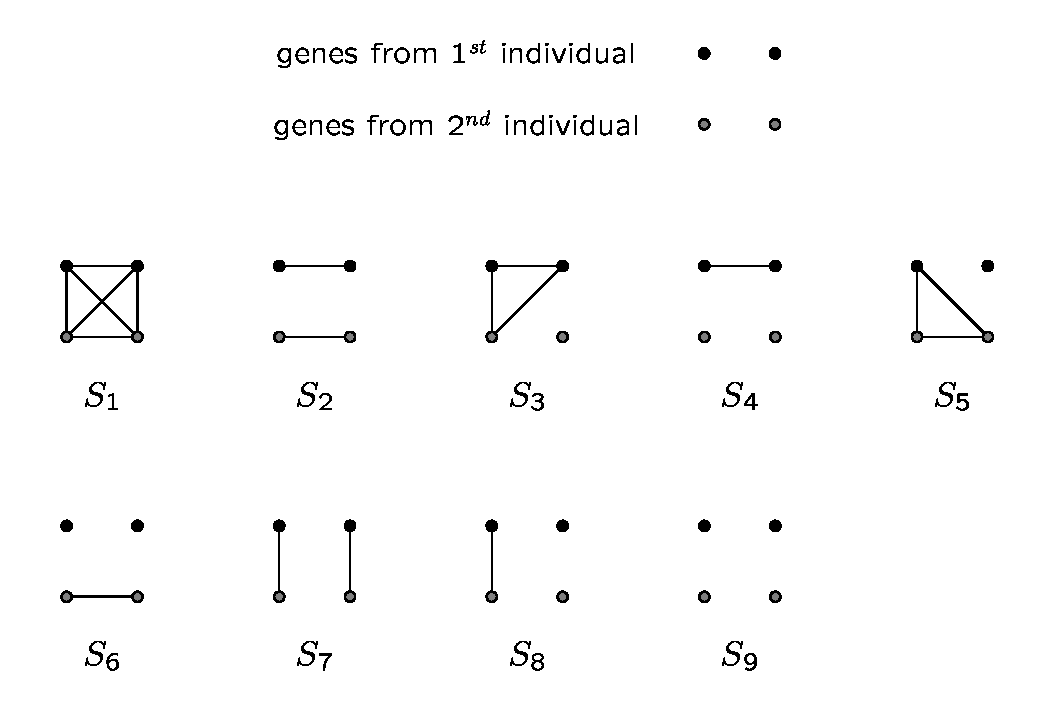
\psfig{file=docfig1.eps,width=4in}
\end{center}
\caption{\label{fig:3}
The nine condensed identity states for 2 individuals}
\end{figure}

Let $\Delta_i=p(S_i)$, the probability of identity state $i$, and
$\boldsymbol{\Delta}$ be the vector of identity state probabilities. To save
space, \Loki does not store estimates of all 9 possible states for each
relative pair.  Instead it calculates two functions of
$\boldsymbol{\Delta}$, twice the kinship coefficient
$2\Phi=2(\Delta_1+\frac{1}{2}(\Delta_3+\Delta_5+\Delta_7)+\frac{1}{4}\Delta_8)$
\ and $\Delta_7+\Delta_1$, as these are the quantities required by most
variance component programs fitting additive and dominance variance
components. Note that these quantities are estimated correctly, even in the
case of inbreeding, but (It is not clear, however, if the
$\Delta_7+\Delta_1$ value is appropriate for the dominance component
in the case of inbreeding, but that is another question{\ldots})

If IBD estimates are requested at many positions (for example, every
centimorgan along a chromosome), the accumulation of the IBD sharing
statistics can account for a significant proportion of the running time.  It
can therefore be advantageous to request \Loki to only collect the sharing
statistics every $n$ iterations.  This has the advantage that the samples
that \textit{are}\ collected are less correlated than if collection is
performed at every iteration.  Obviously if IBD sharing is estimated at only
a few positions (or if unlinked markers are being used), the optimum
strategy may still be to collect estimates at every iteration.  As with
the normal \Loki analyses, the starting iteration and collection frequency
are specified using the START OUTPUT and OUTPUT FREQUENCY commands.

\textbf{N.B.}\ In most cases, pedigree pruning should be turned \emph{off}
in \Prep when IBD estimation is performed (\ref{set_command}).  If not then
individuals may be missing from the output matrices.  Pruning, though useful
in most other cases, should only be left on with IBD estimation if you know
exactly what you are doing!

\subsubsection{Output options}
In contrast to earlier versions of \Loki, only one set of estimates of the IBD
matrices are calculated (at the end of the sampling run).  If \Loki is
interrupted (by the receipt of a signal), it will generate a set of
estimates before quitting.  Note that this can take some time (as the files
can be very large), and it may not always be possible for \Loki to complete
this successfully in time (for example, if the host computer is shutting
down).

Three output formats are currently offered, the default \Loki format, a
MERLIN type format and a SOLAR type format.  The \Loki and MERLIN outputs
are written to a single file (default name \verb+loki.ibd+), which the SOLAR
output is written to a set of files, one file per position
estimated.  These files are written to a directory (default name
\verb+loki_ibd+).  Within this directory, the file names obey the SOLAR
naming scheme, so the file for position 13.4 on chromosome 11 will be called
\verb+mibd.11.13.4.gz+ (if compressed).  This naming scheme can not be
changed.  Note that to properly follow the SOLAR scheme, the chromosome
names should be numeric - this is not enforced by \Loki.

The default file names can be changed using the following commands:
\begin{verbatim}
OUTPUT IBD FILE "myibdfile" # For MERLIN format
OUTPUT IBD DIR "myibd_dir" # For SOLAR format
\end{verbatim}

To reduce the size of the output files, \Loki can compress the output (for
all formats) using gzip (highly recommended!).  This is
done using the following command:
\begin{verbatim}
COMPRESS IBD OUTPUT
COMPRESS OUTPUT IBD # Alternate command format
\end{verbatim}
When this option is used, \verb+.gz+ will be appended to the output file
name, unless the specified name already ends in \verb+.gz+.

\subsubsection{Output Formats}
The output format for the IBD estimates is selected as in the following
examples:
\begin{verbatim}
OUTPUT IBD LOKI # Default output format
OUTPUT IBD MERLIN
OUTPUT IBD SOLAR
\end{verbatim}

The main output to the screen consists only of the iterations count.  The
other output files (notable \verb+loki.out+) are not produced.  The trait
locus code is not invoked at all.

\subsubsection{Default (\Loki) format}
An example fragment of the default output format is shown below:
\begin{verbatim}
Iteration 200

**Linkage group chromosome 1:

**Position = 0
1 1 1 1
2 2 1 1
4 1 0.5 0
4 2 0.5 0
4 4 1 1
5 1 0.5 0
5 2 0.5 0
5 4 0.3975 0.15
5 5 1 1
6 6 1 1
7 1 0.5 0
7 2 0.5 0
7 4 0.485 0.23
7 5 0.4425 0.21
7 7 1 1
\end{verbatim}
As can be seen, the output starts with a small header giving the iteration
number, linkage group and position for which the estimates are for.  This is
then followed by $2\hat{\Phi}$ and $\hat{\Delta_7}$ for each pair of
individuals for whom $\hat{\Phi}>0$.

Note that if family ids are used (so the second form
of the PEDIGREE command is used with \Prep), then there will be an extra
column with the family name before the individual id columns.  

\subsubsection{MERLIN format}
An example fragment MERLIN output format is shown below:
\begin{verbatim}
1 1 0 0 0 1
2 1 0 1 0 0
2 2 0 0 0 1
4 1 0 0 1 0
4 2 0 0 1 0
4 4 0 0 0 1
5 1 0 0 1 0
5 2 0 0 1 0
5 4 0 0.24 0.485 0.275
5 5 0 0 0 1
6 1 0 1 0 0
6 2 0 1 0 0
6 4 0 1 0 0
6 5 0 1 0 0
6 6 0 0 0 1
7 1 0 0 1 0
7 2 0 0 1 0
7 4 0 0.165 0.565 0.27
7 5 0 0.265 0.48 0.255
\end{verbatim}
This format has no header, and the position is given in the $3_{rd}$ column
of the output.  If multiple families are present then the estimates for the
first family at each position are given, then the second family etc.  Unlike
the default format, an output line exists for every pair (even unrelated
pairs).  This can make the output much larger than the default output (even
if compressed).  Three columns of IBD estimates are given, which in the case
of no-inbreeding correspond to $\Delta_9, \Delta_8, \Delta_7$, the
probabilities of the pair sharing 0, 1 and 2 genes IBD.  In the case of
inbreeding, this scheme can not accurately portray the IBD relationships
(and MERLIN as of version 0.9.3 does not try to calculate sharing
probabilities correctly with inbreeding).  In the presence of inbreeding,
\Loki will output values such that the last column ($\Delta_7$) is correct,
and the other columns are adjusted so that if $\Phi$ is calculated using the
formula for non-inbred populations
($\Phi=\frac{1}{2}\Delta_7+\frac{1}{4}\Delta_8$), the correct value for
$\Phi$ (allowing for inbreeding) will be given.  Yes, this is confusing and
no, I don't recommend using this format for inbred families.

As before, if family IDs are used, an extra column of output with the
family name will be outputted.

\subsubsection{SOLAR format}
An example fragment of SOLAR output format is shown below:
\begin{verbatim}
  640   640  1.0000000  1.0000000
  641   641  1.0000000  1.0000000
  773   640  0.5000000  0.0000000
  773   641  0.5000000  0.0000000
  773   773  1.0000000  1.0000000
  643   643  1.0000000  1.0000000
  642   642  1.0000000  1.0000000
  774   643  0.5000000  0.0000000
  774   642  0.5000000  0.0000000
  774   774  1.0000000  1.0000000
  908   640  0.5000000  0.0000000
  908   641  0.0000000  0.0000000
\end{verbatim}
This format has no header, and the position is given in the output filename.
The first 2 columns are the SOLAR IBD IDs, or internal IDs for the pair,
followed by $2\Phi$\ and $\Delta_7$, as with the default format.  The IBD
estimates are always printed to the same precision.  To know the
correspondence between the original IDs and the SOLAR IBD IDs, \Loki needs to
read in two output files from SOLAR, \verb+pedindex.cde+\ and
\verb+pedindex.out+.  These should be put in the current directory.  With
these, \Loki will be able to automatically translate the IDs for SOLAR.
Output lines are only given for related individuals, so the files size tends
to be similar to the default output, and smaller than MERLIN output.
\section{Analysis Scripts and Utility Programs}
\label{scripts}
It is not straightforward to look directly at the output from Loki and make
conclusions about whether there is linkage to a region, how many QTLs are in
the model, what size of QTLs have been found etc.  For this reason, several
perl scripts and small utility programs in C have been supplied with Loki.
These can be used to read the output files from Loki, and produce
either a text report, a selection of columns of data or a graphical view of
the data.  The graphical view of the data requires that \verb+gnuplot+ be installed
on the system.  This is a widely available data plotting utility which
can be downloaded from ftp.dartmouth.edu/pub/gnuplot.  A web page for
\verb+gnuplot+ can be found at http://www.cs.dartmouth.edu/gnuplot.
\subsection{Extracting information on effects: \texttt{loki\_ext.pl}}
The perl script \verb+loki_ext.pl+ can be used to extract information from
the \verb+loki.out+ file such that it can be used by other programs and/or
scripts.  Probably the two most useful applications of this script are to
extract information about QTLs and to extract information about
covariate effects.  To do the former, the script is invoked like this:
\begin{verbatim}
loki_ext.pl -x
loki_ext.pl -x -c2
loki_ext.pl -x -c2 -r20.3:25.7
loki_ext.pl -x -c2 -r20.3
loki_ext.pl -x -c2 -r:25.7
loki_ext.pl -x -i2000
loki_ext.pl -x -i2000:5000
loki_ext.pl -x -i:5000
\end{verbatim}
The -x option specifies an extract operation.  The first example extracts
all QTLs linked to the first linkage group (this is the default) and outputs
the relevant columns to stdout.  The -c option in the second and third
examples indicate that QTLs linked to the second chromosome should be
extracted.  The -r option specifies a range of chromosome positions to look
for QTLs.  Note that either or both of a starting and stopping location can
be given.  The -i option specifies a range of iterations to consider.  As
with the -r option, either or both of a starting and stopping
iteration may be given.

The number of columns output depends on whether the specified linkage group
is 0 (meaning the `unlinked' group) in which case no QTL position
information is output, and whether sex specific maps are being used, in
which case both male and female map positions are output.  For a normal
chromosome with a sex averaged map, the output order is: iteration, map
position, frequency of `1' allele,effect of `12' genotype, effect of `22'
genotype, size of QTL, \% genetic variance due to QTL, \% total variance due
to QTL.  Note that the total variance used to calculate the last column is
the variance after adjusting for any environmental covariates.

To extract information about covariate effects the script is invoked as given below:
\begin{verbatim}
loki_ext.pl -C
loki_ext.pl -D
\end{verbatim}
Using the -C option, loki\_ext simply strips of any QTL columns and the
header from \verb+loki.out+, and outputs the remainder.  The column order is
therefore as given in the header to \verb+loki.out+, and will change
depending on which version of Loki and which output type is being used.
Using the -D option will give a `standardized' set of columns which should
be consistent across different versions and output types.  As before, the
-i option can be used to specify a range of iterations.  The output format
for the -D option is as follows:
\begin{enumerate}
  \item Iteration
  \item No. QTL in model
  \item No. linked QTL. in model
  \item Grand mean
  \item Residual variance
  \item Tau
  \item Total genetic variance
  \item{\ldots}Remainder of non QTL data columns
\end{enumerate}
The output from \verb+loki_ext.pl+ can either be directed to a file and further
analyzed or viewed by programs such as \verb+gnuplot+.  Alternatively the output
can be piped into a program such as \verb+qavg+ to give means and confidence
limits for the columns.
\subsection{Estimating probabilities of linkage to chromosomes: \texttt{count.pl}}
\label{ref_count}
The perl script \verb+count.pl+ reads the files \verb+loki.out+ and
\verb+loki.pos+, because the latter file is not produced by versions of loki
prior to loki\_2.3, this scripts only works with output produced by
loki\_2.3 or later.  The file is invoked as follows:
\begin{verbatim}
count.pl [-q] [-f outfile] [-p posfile] [-i start:stop] [-b bin-size] [-c step]
\end{verbatim}
where the -f and -p options allow the specification of
alternative input files rather than the defaults of \verb+loki.out+ and
\verb+loki.pos+.  By default the script displays on the screen the iteration count it has
reached, this can be turned off using the -q (for quiet) option.
As with \verb+loki_ext.pl+, a range of iterations can be
specified using the -i option.  Note that unlike \verb+loki_ext.pl+, the
iteration count is from the first iteration in the file, which may not be
the first sampling iteration.  The output of \verb+count.pl+ looks something
like this:
\begin{verbatim}
----------------------------------------------
Model: Q(1) = QTL + AGE_AT_EXAM + SX
Iterations: 9470

Linkage group    Count   Prop. linked    BF
----------------------------------------------
unlinked          9470     1.00000     1.00116
chrom16            173     0.01827     0.12015   132.23   24.53cM
chrom19           5022     0.53031     4.09343     1.02   90.32cM

QTL number       0      1      2      3      4      5      6
--------------------------------------------------------------
Overall       0.0000 0.0024 0.1122 0.4181 0.3219 0.1094 0.0314
unlinked      0.0000 0.0720 0.2492 0.3918 0.2270 0.0492 0.0108
chrom16       0.9817 0.0177 0.0005 0.0000 0.0000 0.0000 0.0000
chrom19       0.4697 0.5087 0.0207 0.0010 0.0000 0.0000 0.0000
\end{verbatim}
The script produces information about the model used and the total number of
iterations measured (this will be the total iteration count less the
iterations discarded at the beginning).  Then follows a table giving for
each linkage group the number of iterations when that linkage group contains
a QTL, the same as a proportion, and an estimate of the Bayes Factor (BF)
for linkage to the chromosome.  This is calculated in the following way. For
each linkage group, the prior probability $p$ of linkage for any single QTL
is $m/t$, where $m$ is the map length of the chromosome and $t$ is the total
map length of the genome.  These values should be set in the parameter file,
and are printed in the header of \verb+loki.out+.  If sex specific maps are
used (Section \ref{sex_spec}), then $p$ is calculated as
$(m_f+m_m)/(t_f+t_m)$, where $m_f$ and $m_m$ are the male and female
chromosome map lengths and $t_f$ and $t_m$ are the male and female total
genome lengths.  For a given iteration, the prior probability that at least
1 QTL is linked to a chromosome is $1-(1-p)^n$, where $n$ is the number of
QTLs in the model at that iteration.  The posterior probability is either $1$
or $0$ depending on whether or not a QTL is linked.  The posterior/prior
ratio for each linkage group is then averaged over iterations to give the
Bayes Factor. An equivalent calculation is performed for the unlinked
region, where its map length is defined as the amount of total genome
remaining after subtraction of all fitted chromosomes.  After this table is
printed the distribution of QTL number in the model, and the same
information calculated for each linkage group separately.  The last two
columns (or last four columns if a sex specific map is being used) give the
maximum Bayes Factor obtained when each chromosome is split into small bins,
and the location of the bin having the maximum Bayes Factor.  The bin size
defaults to 1cM, but this can be altered using the -b option.  This calculation
of the Bayes Factors for the small regions is the same as performed by
\verb+dist.pl+ described below.

\subsection{Estimating probabilities of linkage to small regions: \texttt{dist.pl}}
The perl script \verb+dist.pl+ reads the same output files as
\verb+count.pl+ (Section \ref{ref_count}) and produces a table with the
estimated Bayes Factor for linkage at a series of locations along the fitted
chromosomes.  If \verb+gnuplot+ is installed, then the script can directly produce
graphs on the screen or produce postscript versions of the graphs. For much
of what is described below, it is assumed that \verb+gnuplot+ is installed and your
PATH is set correctly so it can be found. The calculation of the Bayes
Factor estimate is performed in the same way as described for
\verb+count.pl+, but instead of treating each chromosome in its entirety
the chromosome is split into equally sized bins with the Bayes Factor being
estimated separately for each bin.  The script has numerous options which
are described below.  If run without options it will produce a graph on the
screen showing the estimated Bayes Factors along each chromosome in turn
using a bin size of 1cM.  Available options are:
\begin{verbatim}
  -c n           only consider the nth linkage group
  -b n           set bin size to n (cM)
  -d name        use name as the base name for temporary files.  Don't delete
                 temporary files after use.
  -f file        select which output file to read from (defaults to loki.out)
  -p file        select which position file to read from (defaults to loki.pos)
  -o file        write postscript output to file
  -q             do not invoke gnuplot
  -C             produces color postscript plots (only has effect with -o)
  -i start:stop  select range of iterations
\end{verbatim}
The temporary files, which can be examined by use of the \verb+-d+ option
consist of a \verb+gnuplot+ control file and a data file.  If the script was
invoked as \verb+dist.pl -d junk+, the control file would be called
\verb+junk+ and the data file \verb+junk.dat+.  Typing \verb+gnuplot junk+
should reproduce the graphs.
\subsection{Estimating marker allele frequencies: \texttt{freq.pl}}
\label{lab.freq2}
This script takes the raw marker allele frequency realizations produced
using the command OUTPUT FREQUENCY "freqfile" (Sections \ref{lab.freq1} and
\ref{lab.freq}), and produces an allele frequency estimate for each allele.
Optionally it also calculates confidence intervals for the estimates.
Example usages follow:
\begin{verbatim}
freq.pl freqfile
freq.pl -p 0.025 freq.dat
\end{verbatim}
The second form would instruct the script to produce the 2.5\% and 97.5\%
confidence limits for the estimates.  The output from the script is fairly
self explanatory; the second form of the script produces output like this:
\begin{verbatim}
D1S1597
   3        0.2372 (0.2048-0.2759) 
   4        0.0029 (0.0004-0.0084) 
   5        0.0128 (0.0058-0.0219) 
   6        0.4530 (0.4121-0.4888) 
   7        0.2512 (0.2186-0.2829) 
   8        0.0429 (0.0291-0.0579) 
D1S1612
   2        0.0027 (0.0003-0.0080) 
   4        0.1368 (0.1138-0.1669) 
   5        0.3374 (0.3030-0.3754) 
   6        0.1248 (0.1018-0.1485) 
   7        0.2568 (0.2235-0.2904) 
   8        0.0156 (0.0076-0.0261) 
   9        0.1190 (0.0974-0.1436) 
   10       0.0027 (0.0004-0.0068) 
   11       0.0041 (0.0009-0.0087) 
\end{verbatim}
Each marker is presented in turn, followed by the alleles, frequency
estimate and confidence intervals if requested.
\subsection{Obtaining column averages - \texttt{qavg}}
This is a small utility program which will quickly calculate averages and
provide summary statistics about column data.  If invoked with a file name
it will read the file and print summary information about each column in the
file, otherwise it will read from standard input.  The basic information it
provides is the mean, standard deviation, no. records and range of each
column.  An example output follows:
\begin{verbatim}
Col 1 - Mean = 51000 SD = 28869.7 n = 20001 Range 1000 -> 101000
Col 2 - Mean = 1.05272 SD = 0.250372 n = 20001 Range 0.202457 -> 1.96742
Col 3 - Mean = 3.27452 SD = 0.369947 n = 20001 Range 2.11931 -> 4.73246
Col 4 - Mean = 2.59041 SD = 0.448593 n = 20001 Range 0.48428 -> 4.04446
Col 5 - Mean = 65.2765 SD = 1.38383 n = 20001 Range 56.5785 -> 72.829
Col 6 - Mean = -0.412581 SD = 0.183528 n = 20001 Range -1.13458 -> 0.364772
Col 7 - Mean = -0.317538 SD = 0.186775 n = 20001 Range -1.07009 -> 0.483818
Col 8 - Mean = -1.04013 SD = 0.178181 n = 20001 Range -1.68759 -> -0.240899
\end{verbatim}
If the data are log transformed and it is wished that the averaging is
performed on the original scale (for example, if the data are log
likelihoods), then this can be achieved using the -l option \IE 
\verb+qavg -l+.

In addition, \verb+qavg+ can give empirical confidence limits using the -p
flag; the command \verb+qavg -p0.025+ will give the 2.5\% and 97.5\% limits.
This option will also make the program output the first, second and third
quartiles (Q1, Q2, Q3), and an empirical `p-value'.  This latter is
calculated as follows.  If the mean of a column is $>0$, then the p-value is
the proportion of data items which are $<=0$, and visa versa when the mean
is $<0$.  This measure is intended as a quick aid to assessing the
significance of covariate estimates.  An example output using this option
follows:
\begin{verbatim}
Col 1 - Mean = 51000 SD = 28869.7 n = 20001 Range 1000 -> 101000
     Q1 = 26000, Q2 = 51000, Q3 = 76000, 2.5% Lim = 3500 -> 98500, p = 0
Col 2 - Mean = 1.05272 SD = 0.250372 n = 20001 Range 0.202457 -> 1.96742
     Q1 = 0.882824, Q2 = 1.06423, Q3 = 1.22872, 2.5% Lim = 0.53308 -> 1.51554, p = 0
Col 3 - Mean = 3.27452 SD = 0.369947 n = 20001 Range 2.11931 -> 4.73246
     Q1 = 3.0134, Q2 = 3.25833, Q3 = 3.52037, 2.5% Lim = 2.59481 -> 4.03333, p = 0
Col 4 - Mean = 2.59041 SD = 0.448593 n = 20001 Range 0.48428 -> 4.04446
     Q1 = 2.34131, Q2 = 2.62509, Q3 = 2.88829, 2.5% Lim = 1.60588 -> 3.38831, p = 0
Col 5 - Mean = 65.2765 SD = 1.38383 n = 20001 Range 56.5785 -> 72.829
     Q1 = 65.0735, Q2 = 65.3966, Q3 = 65.6771, 2.5% Lim = 61.2552 -> 68.02, p = 0
Col 6 - Mean = -0.412581 SD = 0.183528 n = 20001 Range -1.13458 -> 0.364772
     Q1 = -0.537258, Q2 = -0.411998, Q3 = -0.29009, 2.5% Lim = -0.775722 -> -0.0502515, p = 0.0121494
Col 7 - Mean = -0.317538 SD = 0.186775 n = 20001 Range -1.07009 -> 0.483818
     Q1 = -0.443942, Q2 = -0.318493, Q3 = -0.190569, 2.5% Lim = -0.677856 -> 0.0481646, p = 0.0456977
Col 8 - Mean = -1.04013 SD = 0.178181 n = 20001 Range -1.68759 -> -0.240899
     Q1 = -1.16117, Q2 = -1.03919, Q3 = -0.919638, 2.5% Lim = -1.38943 -> -0.691617, p = 0
\end{verbatim}
The use of this option requires the program to hold all of the data in
memory and sort it which adds to the computational requirements of the
script, so it should not be used on very large datafiles.
\section{Acknowledgements}
The author is grateful to Warwick Daw for testing versions and for
helpful discussion and comments.  This work was previously supported by NIH Grant
GM46255 and is currently supported by NIH grant GM58757.
\bibliography{master}
\bibliographystyle{ajhg}
\end{document}
